\section{Mapping classical phenotypes}
Perfect timing of germination is required to encounter optimal conditions for plant survival and it 
is the result of a complex interaction between molecular processes, seed characteristics and 
environmental cues. To detangle these processes we made use of natural genetic variation present in 
an Arabidopsis thaliana Bayreuth x Shahdara RIL population. For a detailed analysis of the germination 
response we characterized rate, uniformity and maximum germination and discussed the added value of 
such precise measurements. The effects of after-ripening, stratification and controlled deterioration 
as well as the effect of salt (NaCl), mannitol, heat, cold and ABA with and without cold stratification 
were analyzed for these germination characteristics. Seed morphology (size, length) of both dry and 
imbibed seeds were quantified by using image analysis. For the overwhelming amount of data produced 
in this study we developed new approaches to perform and visualize high throughput QTL analysis. 
We show correlation of trait data, (shared) QTL positions and epistatic interactions. The detection 
of similar loci for different stresses indicate that often the molecular processes regulating 
environmental responses converge into similar pathways. 7 major QTL hotspots were confirmed using a 
HIF approach. QTLs co-locating with previously reported QTLs and well characterized mutants are 
discussed. A new connection between dormancy, ABA and a cripple mucilage formation due to a natural 
occurring mutation in the MUM2 gene is proposed and this is an interesting lead for further research 
on the regulatory role of ABA in mucilage production and its multiple effects on germination parameters.

\subsection{Background}
Colonizing plants are subject to a wide variety of environmental conditions. For successful adaptation 
to new habitats the timing of developmental transitions is especially important. Seed germination is 
one of these important transitions as it determines the seasonal environment experienced in further 
plant life \cite{Huang:2010}. Natural populations that develop under distinct environmental conditions 
may reveal genetic adaptation, which can be used to disentangle the signaling routes that are involved. 
Seed germination is described by three phases of water uptake. In phase I the seeds imbibes and 
reinitiates metabolic processes followed by a lag phase (phase II). Further water uptake results in 
protrusion of the radicle through the testa and endosperm (phase III). The moment of radicle 
protrusion through the endosperm is considered to be the moment of germination sensu stricto 
\cite{Finch-Savage:2006}. To characterize the genetic variation of germination related traits we 
focused on the effect of the environment that a seed perceives during germination rather than the 
effect of the environment during maternal plant growth, which has been the subject of other 
studies \cite{Dechaine:2009, Elwell:2011}. 

\begin{figure}[h!]
  \centering
  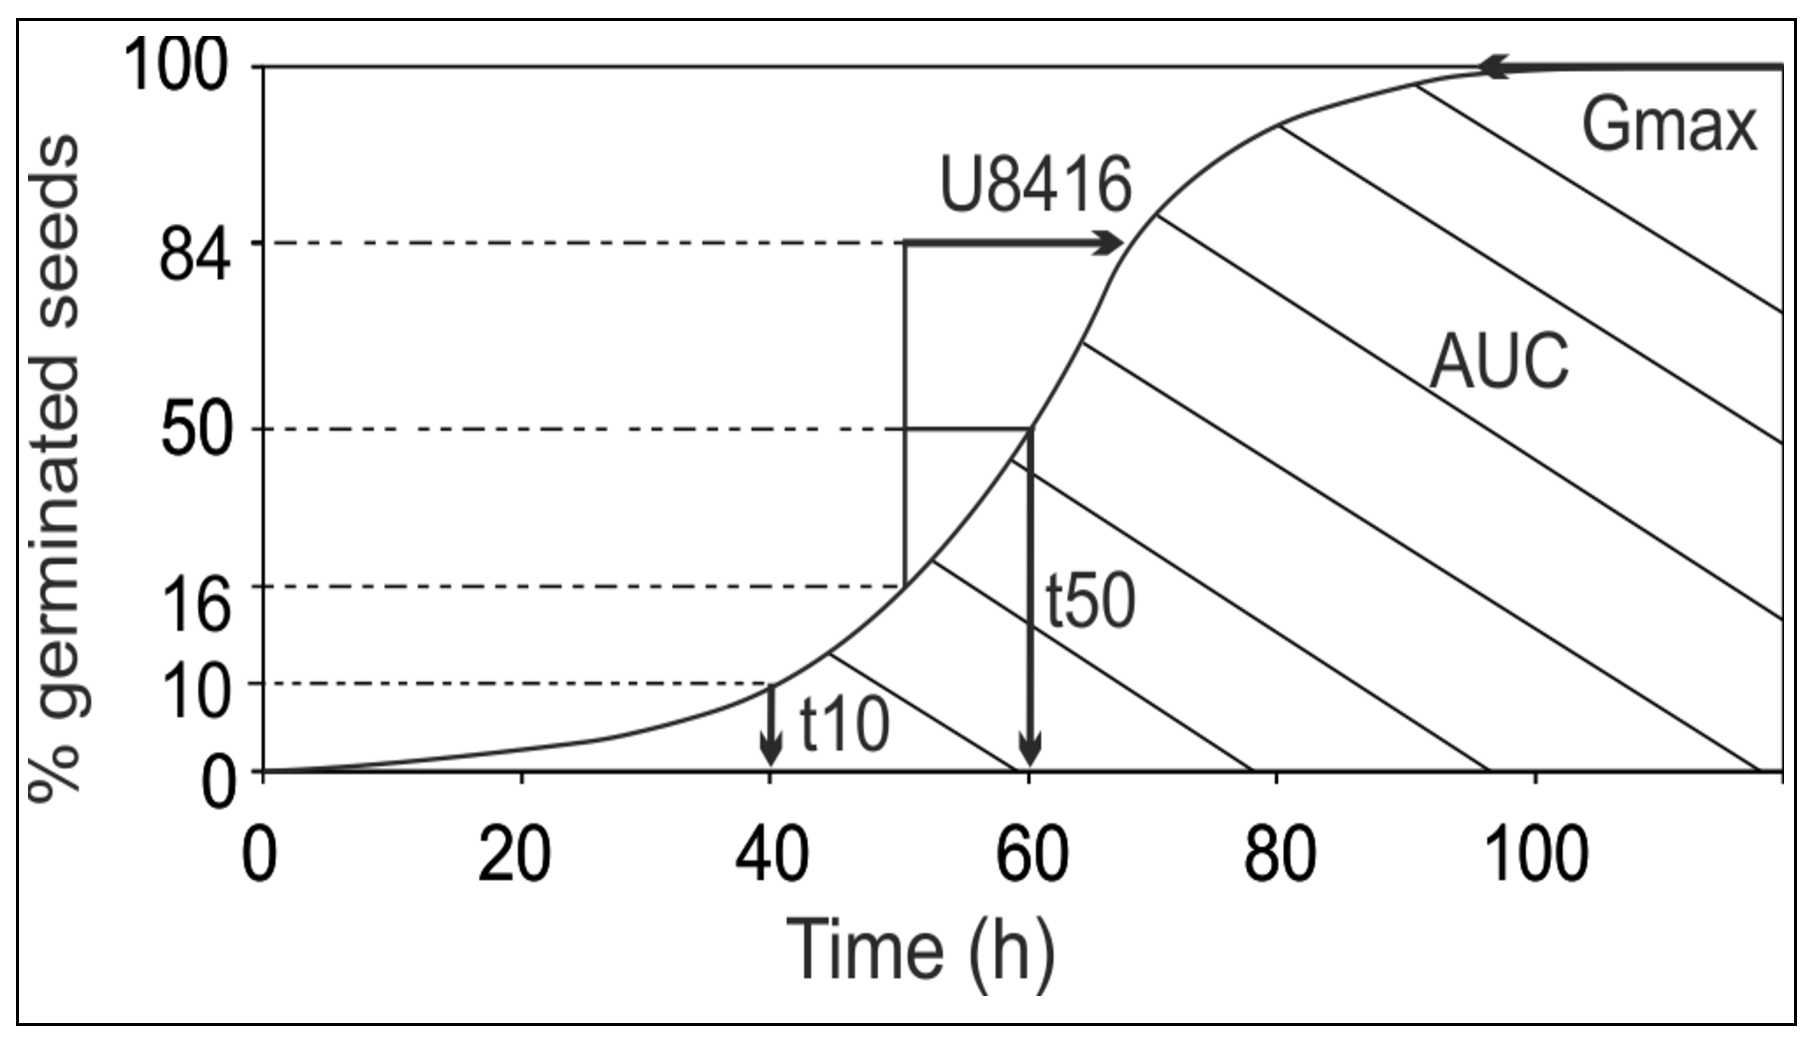
\includegraphics[keepaspectratio,scale=0.30]{eps/image_3_1_1.eps}
  \caption[Germination curve.]
    {Germination curve.}
\end{figure}

Seed content (e.g. oil) is often used as commodity and modifications to the content can therefore be 
regarded as seed quality parameters as well. To prevent confusion we will use the term seed performance 
to indicate that the focus of our study was restricted to seed germination characteristics.

The production of high quality crop seed not only entails knowledge about maternal plant growth, 
harvesting and storage of seeds, but also of germination conditions \cite{Rivero-Lepinckas:2006}. 
To obtain better germination and field performance, many seed companies rely on enhancement methods, 
such as seed priming and coating and/or pelleting, but these methods are reaching their limits. 
Dissecting the molecular mechanisms underlying seed germination and its tolerance to the environment 
may unlock the full genetic potential and enable targeted breeding for seed performance. In this study 
we used a recombinant inbred line (RIL) population derived from two Arabidopsis thaliana ecotypes: 
Bayreuth (Bay-0) which originates from a fallow land habitat in Germany and Shahdara (Sha) which 
grows at high altitude in the Pamiro-Alay mountains in Tadjikistan \cite{Loudet:2002}. The Bay-0 x 
Sha RIL population has been used in many previous studies to map QTL positions for root morphology 
\cite{Loudet:2005, Reymond:2006}, anion content \cite{Loudet:2003a}, nitrogen use efficiency 
\cite{Loudet:2003b}, cell wall digestibility \cite{Barriere:2012}, carbohydrate content 
\cite{Calenge:2006}, sulfate content \cite{Loudet:2007}, leaf senescence \cite{Diaz:2006}, 
morning-specific growth \cite{Loudet:2008} and cold-dark germination \cite{Meng:2008}. We have used 
the natural variation present in this RIL population to map the response of germination characteristics 
to environmental conditions to which a seed is exposed.

\begin{table}[h]
  \centering
  {\footnotesize
  \begin{tabular}{  l  l  l  l  l  l }
    \hline
    {\bf Trait} & {\bf Gmax} & {\bf AUC} & {\bf T50}& {\bf T10}& {\bf A8416}\\
    \hline
    AR.NS           & 0.82 & 0.97 & 0.86 & 0.79 & 0.82 \\
    AR.NS.Cold      & 0.51 & 0.77 & 0.73 & 0.66 & 0.48 \\
    AR.NS.Mannitol  & 0.61 & 0.79 & 0.70 & 0.55 & 0.62 \\
    AR.NS.NACL      & 0.90 & 0.94 & 0.80 & 0.76 & 0.43 \\
    AR.WS           & 0.63 & 0.19 & 0.78 & 0.72 & 0.72 \\
    AR.WS.NACL      & 0.91 & 0.93 & 0.86 & 0.78 & 0.70 \\
    Fresh.NS        & 0.92 & 0.94 & 0.81 & 0.70 & 0.76 \\
    Fresh.WS        & 0.40 & 0.81 & 0.87 & 0.84 & 0.76 \\
    \hline
  \end{tabular}
  }
  \caption[Heritability Overview]{Overview of the broad sense heritability scores. Included are those traits for which different blocks 
          were tested (Trait code descriptions can be found in Table \ref{table:codes})}
\end{table}

Freshly harvested viable Arabidopsis seeds often don't germinate even when placed under conditions 
favorable for germination. This event, called primary dormancy, is shown to be subject to natural 
variation \cite{Bentsink:2010}. In many Arabidopsis ecotypes, this primary dormancy is released after 
a period of dry storage at room temperature. Another dormancy breaking treatment is cold stratification 
were seeds are imbibed in water and stored at 4\degree C in the dark for four days before putting them into 
optimal conditions for germination \cite{Finch-Savage:2006}. Unfavorable conditions during seed 
germination may result in a changed rate or even failure of germination. In Arabidopsis, it has been 
shown that the responsiveness to temperature is closely related to the level of after-ripening 
\cite{Tamura:2006}. High salt concentrations induce osmotic stress and ion toxicity resulting in both 
a delay and reduction of maximum germination \cite{Galpaz:2010}. Often, these different environmental 
stresses are interconnected and will cause osmotic and associated oxidative stress \cite{Zhu:2002, 
Chinnusamy:2004}. The plant hormone Abscisic Acid (ABA) plays a predominant role in plant 
responses to different environmental stresses and can activate various signal transduction pathways 
leading to a global change in transcription \cite{Finkelstein:2002, Xiong:2002}. Exogenous application 
of ABA during germination results in a distinction between testa and endosperm rupture. At certain 
concentrations the testa will rupture but germination sensu stricto (radicle protrusion through the 
endosperm) will be inhibited. This phenomenon, caused by reduced weakening of the endosperm cap, is 
the consequence of a complex interplay between ABA, GA and ethylene signals \cite{Linkies:2009}. 
In this report, we determined germination sensu stricto for primary dormancy in freshly harvested seeds, 
germination of fully after- ripened seeds with and without a preceding cold stratification period 
(see material and methods for conditions), and germination under various stress conditions (low/high 
temperature, salt/osmotic stress and ABA) to assess natural  variation in the Bay-0 x Sha RIL population. 
Additionally, seed morphology (size and length) and flowering time were phenotyped as they have been 
shown to be strong determinants of plant trait variation \cite{Elwell:2011, Chiang:2009, Orsi:2009}. 
We correlated these traits to our germination related traits to evaluate 
possible causality. In total this analysis resulted in 327 trait scores over different harvests. 
Evaluation of these high numbers of phenotypes demanded methods of QTL analysis that extended beyond 
mapping of individual traits and that allowed comprehensive and comprehensible visualization.

\definecolor{C1}{HTML}{2800FF}
\definecolor{C2}{HTML}{8CB4E1}
\definecolor{C3}{HTML}{B4DCE1}
\definecolor{C4}{HTML}{5096B4}

\definecolor{C5}{HTML}{F0F0A0}
\definecolor{C6}{HTML}{FFFF64}

\definecolor{C7}{HTML}{E6DCF0}
\definecolor{C8}{HTML}{B4A0C8}

\definecolor{C9}{HTML}{D2E6B4}
\definecolor{C10}{HTML}{78B478}
\definecolor{C11}{HTML}{78963C}

\definecolor{C12}{HTML}{FAE6DC}
\definecolor{C13}{HTML}{FABE8C}
\definecolor{C14}{HTML}{FA8C32}

\definecolor{C15}{HTML}{DCDCC8}
\definecolor{C16}{HTML}{C8BE96}

\definecolor{C17}{HTML}{E6B4B4}
\definecolor{C18}{HTML}{DC9696}

\definecolor{C19}{HTML}{96FF96}
\definecolor{C20}{HTML}{96C800}
\definecolor{C21}{HTML}{C8C800}

\begin{table}[h]
  \tiny
  \centering
  \begin{tabular}{ | l | c | l | l | p{4cm} | l | }
    \hline
    {\bf Trait Group}    & {\bf Stratification} & & {\bf Harvest} & {\bf Description}                                                                                          & {\bf Codes}               \\
    \hline
    Germination               & N & \cellcolor{C1} & ABCD          & After ripened seed germination                                                                                           & AR.NS                     \\
    \hline
    After ripening            & N & \cellcolor{C2} & ABCD          & Delta between freshly harvested seed germination and after-ripened seed germination                                      & AR.NS - Fresh.NS          \\
    \hline
    Fresh                     & Y & \cellcolor{C3} & ABCD          & Delta between freshly harvested seed germination and freshly harvested seed germination                                  & Fresh.WS -Fresh.NS        \\
    \hline
    AR                        & Y & \cellcolor{C4} & ABCD          & Delta between after-ripened seed germination and after-ripened  seed germination                                         & AR.WS - AR.NS             \\
    \hline
    NaCl                      & N & \cellcolor{C5} & ABCD          & Delta between after-ripened seed germination on 100 mM NaCl and after-ripened  seed germination on water                 & AR.NS - NaCl.             \\
    NaCl                      & Y & \cellcolor{C6} & ABCD          &                                                                                                                          & AR.WS - NaCl.WS.          \\
    \hline
    Mannitol                  & N & \cellcolor{C7} & AD            & Delta between after-ripened seed germination on -0.5 mP Mannitol and after-ripened seed germination on water             & AR.NS - AR.Mann.NS.       \\
    Mannitol                  & Y & \cellcolor{C8} & AD            &                                                                                                                          & AR.WS - AR.Mann.WS.       \\
    \hline
    Cold Fresh                & N & \cellcolor{C9} & D             & Delta between freshly harvested seed germination at 10\degree C and freshly harvested seed germination at 20\degree C    & Fresh.NS - Fresh.Cold.NS  \\
    Cold                      & N & \cellcolor{C10} & AD            & Delta between after-ripened seed germination at 10\degree C and after-ripened seed germination at 20\degree C            & AR.NS - AR.Cold.NS        \\
    Cold                      & Y & \cellcolor{C11} & D             &                                                                                                                          & AR.WS - AR.Cold.WS        \\
    \hline
    Heat Fresh                & N & \cellcolor{C12} & D             & Delta between freshly harvested seed germination at 30\degree C and after-ripened seed germination at 20\degree C        & Fresh.NS - Fresh.Heat.NS  \\
    Heat                      & N & \cellcolor{C13} & D             & Delta between after-ripened seed germination at 30\degree C and after ripened seed germination at 20\degree C            & AR.NS - AR.Heat.NS        \\
    Heat                      & Y & \cellcolor{C14} & D             &                                                                                                                          & AR.WS - AR.Heat.WS        \\
    \hline
    CD*                       & N & \cellcolor{C15} & D             & Delta between after-ripened seed germination after controlled detoriation and after-ripened seed germination on water    & AR.NS - AR.CD.NS          \\
    CD*                       & Y & \cellcolor{C16} & D             &                                                                                                                          & AR.WS - AR.CD.WS          \\
    \hline
    ABA                       & N & \cellcolor{C17}  & D             & Delta between after-ripened seed germination with  0.5 $\mu$M ABA and after-ripened seed germination on water            & AR.NS - AR.ABA.NS         \\
    ABA                       & Y & \cellcolor{C18}  & D             &                                                                                                                          & AR.WS - AR.ABA.WS         \\
    \hline
    Seed size                 & N & \cellcolor{C19} & ABD           & Seed size and length of dry seeds                                                                                        & Size.Area                 \\
    Seed size, imbibed        & N & \cellcolor{C20} & ABD           & Seed size of imbibed seeds                                                                                               & Size.imbibed              \\
    Flowering time            & N & \cellcolor{C21} & ABD           & First open flower in long day (16D/8N) conditions                                                                        & FTLD                      \\
    \hline
  \end{tabular}
  \caption[Trait codes]{Overview of traits in this study and the harvest(s) used for the measurement. The indicated color-code 
          is used in all figures throughout this paper. For each mentioned experiment $G_{max}$, AUC, $t_{50}$, $t_{10}$ and $U_{8416}$ were determined.}
  \label{table:codes}
\end{table}

\begin{figure}[h!]
  \centering
  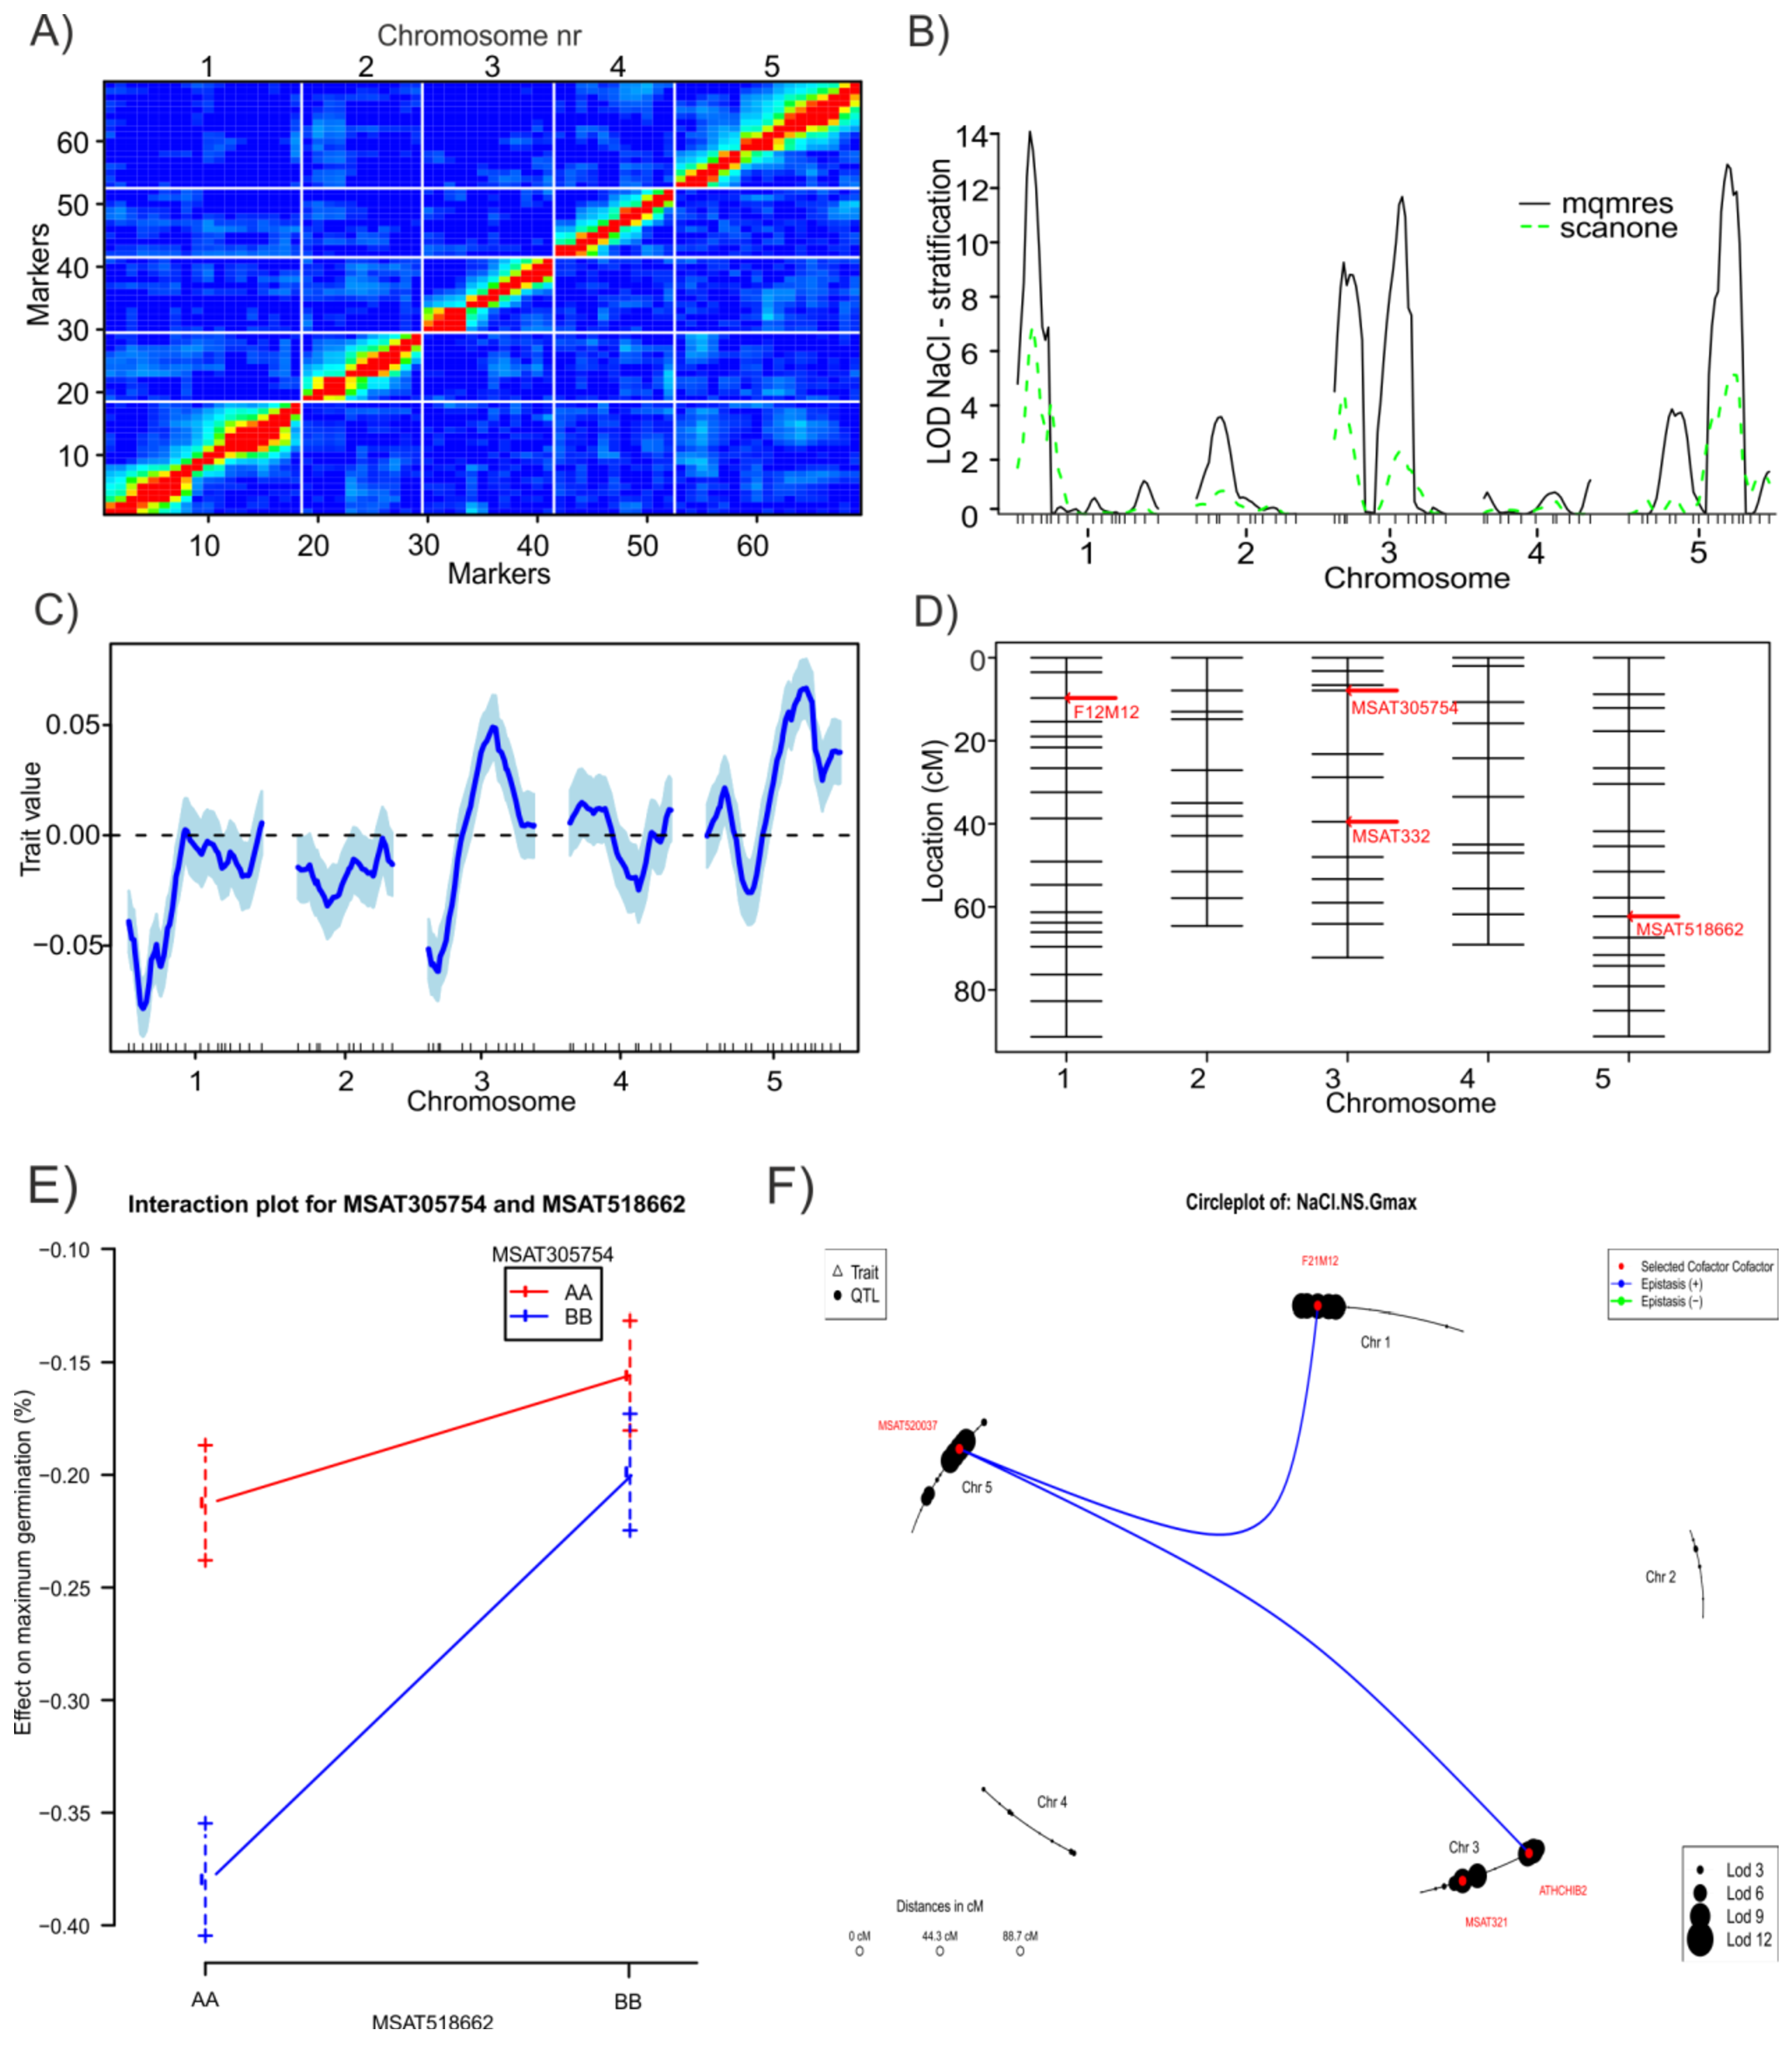
\includegraphics[keepaspectratio,scale=0.30]{eps/image_3_1_2.eps}
  \caption[Generated Output.]{R/QTL output for the effect of 100mM NaCl on the maximum germination without 
          stratification. A) Pairwise recombination fractions; B) Phenotype distribution histogram without 
          normalization ; B) LOD profile comparison between MQM and Haley-Knott (scan-one) interval mapping; 
          C) Genome wide additive effect based on raw phenotype data D) Genetic map showing the significant 
          QTL markers; E) Interaction plot showing the effect size comparison between marker MSAT305754 and 
          MSAT518662 at the Sha (AA) and Bay-0 (BB) alleles; F) Circle plot showing interactions between 
          all significant markers.}
          \label{fig:generatedoutput}
\end{figure}

Analysis of natural variation that is captured in well-defined recombinant inbred populations has 
shown to be a powerful tool to detect important loci that influence the traits under study 
\cite{Alonso-Blanco:2009}. To uncover the loci with genetic variation a statistical framework is 
needed. For this, any programming language can be used which supports statistics. In the life sciences 
the statistical language R is often the prime candidate. R is open source, contains the latest in 
statistical analysis methods and has a large community for help and support (http://www.r-project.org/). 
Furthermore, it has the R/qtl package \cite{Broman:2003}, which contains an array of different 
QTL mapping methods, including Single Marker Mapping, Interval Mapping and Multiple QTL Mapping (MQM) 
\cite{Arends:2010}. Although all possibilities to perform a detailed QTL analysis including data 
preprocessing and output formatting are present in R, it requires extensive knowledge of the R-syntax 
to combine all necessary steps in a single analysis protocol that can loop through hundreds or 
thousands of traits. 

We present a script that can perform these tasks. This type of automated analysis combined with 
efficient data visualization is a necessary step to keep up with the increasing rate of biological 
data production. For using single trait mapping the effect of a certain treatment, e.g. germination 
at high temperature, must be corrected by the germination characteristics under control conditions. 
Here, we subtracted the observed germination under stress conditions from values for germination 
under control conditions. This correction can lead to complicated interpretation, especially when the 
environment under study affects loci with already strong effects under control conditions. Further, 
it can reduce statistical power due to summation of the error components. Therefore we performed an 
additional analysis using a QTL by environment (QTLxE) approach \cite{Vargas:2006, Moreau:2004}. 
Instead of considering individual responses, one can then treat the stress conditions as a set of 
environmental perturbations and evaluate a single trait (such as germination percentage). Because 
several environments are taken into account simultaneously, the statistical power to detect loci 
that are affected by several environments increases and interpretation becomes more intuitive as the 
need for correcting the stress response by the control response is eliminated \cite{Boer:2007}.

The Bay-0 x Sha RIL population consists of 420 lines that were genotyped in the F6. This relatively 
low degree of inbreeding provoked residual heterozygosity present at almost all genome positions. 
This residual heterozygosity can be used to confirm QTL positions, as it provides a possibility to 
study both parental alleles at the locus of interest in an elsewhere homozygous background. 
In contrast to conventional near isogenic lines (NILs) the genetic background of heterogeneous 
inbred lines (HIFs) consist of a mix of the two parental genomes. The availability of a genome wide 
set of HIF lines for the Bay-0 x Sha RIL population provides a fast and accurate means to confirm 
detected QTL loci.

\subsection{Results}

\subsubsection{Single trait QTL mapping}
To evaluate the response of germination to a certain treatment, we first subtracted the observed 
germination at test conditions from germination at the proper control conditions. For example, the 
effect of NaCl on germination after cold stratification is determined by subtracting Gmax on 
NaCl from Gmax on water. This subtraction was reversed for the rate and uniformity parameters to 
correct the reversed nature of these parameters (e.g. slower germination results in a larger t10 
and t50). Table \ref{table:codes} gives an overview of all corrections that have been applied. 

\begin{figure}[h!]
  \centering
  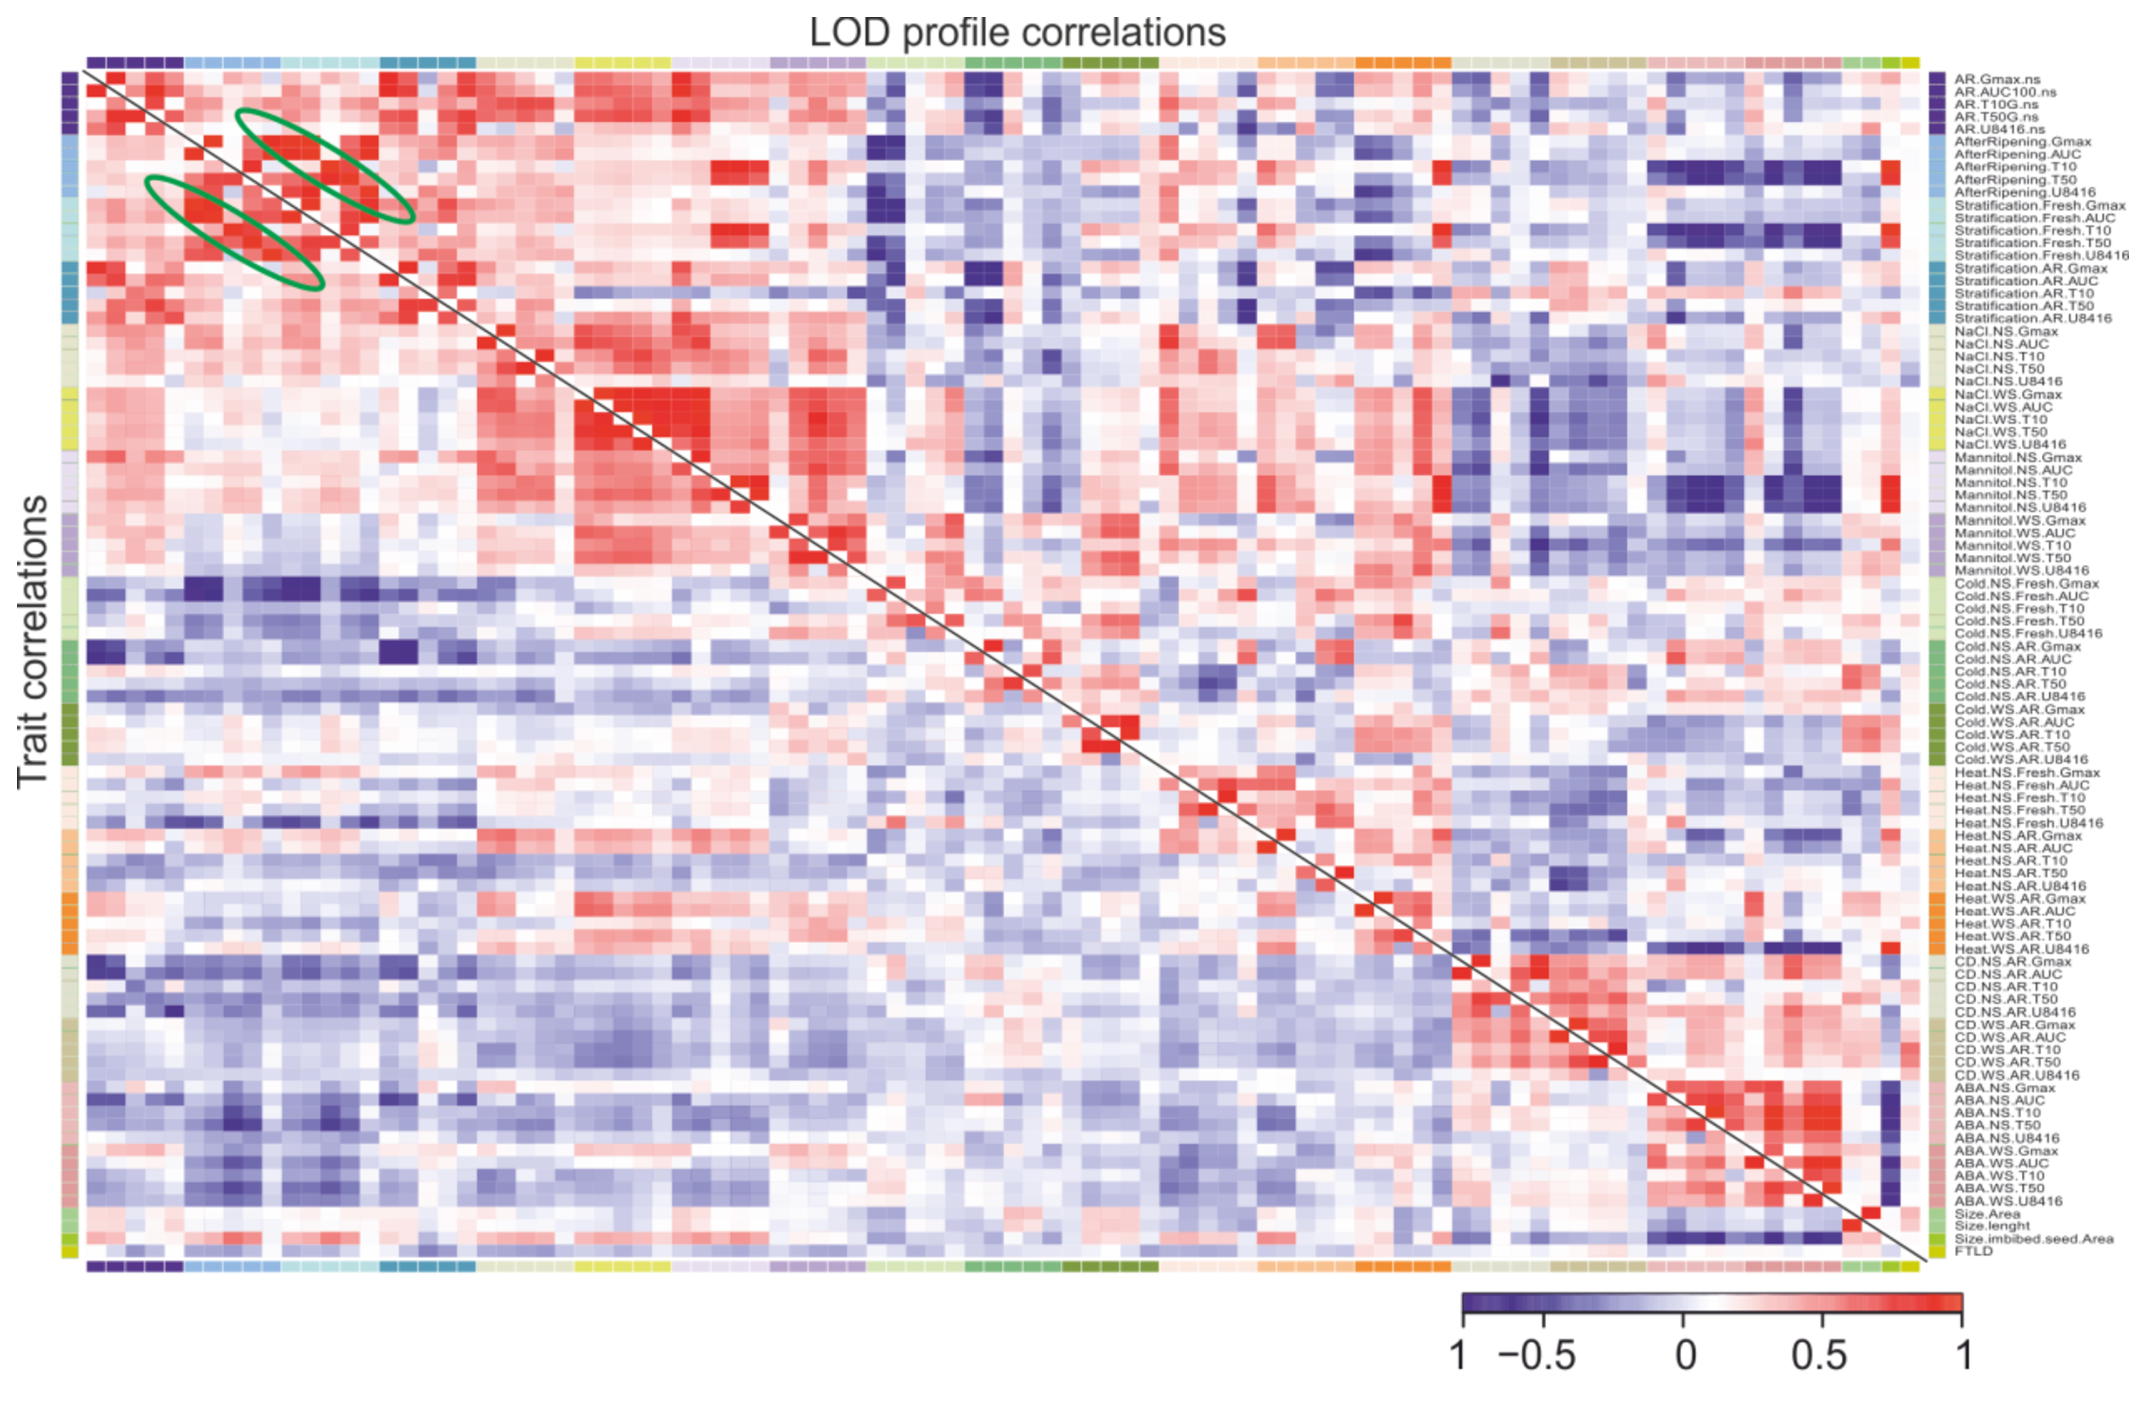
\includegraphics[keepaspectratio,scale=0.30]{eps/image_3_1_3.eps}
  \caption[Heatmap of correlation.]{Correlation between all trait values (bottom left panel) and between 
          all LOD profiles (top right panel). Traits are indicated by the color code depicted in Table \ref{table:codes}. 
          Green circles indicate an example of the close correlation between "after-ripened" and "fresh 
          with stratification" trait values.}
\end{figure}

An analytical protocol was designed, using the popular R/qtl package of R to analyze trait data of 
recombinant inbred populations with the multiple QTL model approach \cite{Arends:2010}. When 
performing a detailed QTL analysis it is important that several steps are performed or checked. 
Missing genotypic data is imputed and a recombination frequency plot is generated (Fig. \ref{fig:generatedoutput}A). In 
the next step, quality of the trait data is investigated. Outliers are detected and removed using 
a Zscore transformation with a user defined threshold. As an extra control the results of MQM mapping 
were always compared to standard interval mapping, using the parametric model with Haley Knott 
regression \cite{Haley:1992} (Fig. \ref{fig:generatedoutput}B). The whole genome additive effect was estimated based 
on the non-transformed data as half the difference between the phenotypic averages for the two 
homozygotes (Fig. \ref{fig:generatedoutput}C).

R/qtl MQM uses a backward elimination of cofactors. As a rule of thumb one can select a maximum of 
$N-20$ initial cofactors with this procedure \cite{Handbook:Jansen:2007}, with $N$ being the number of lines in 
the RIL population. In our script, a cofactor file can be provided with the selection of the initial 
cofactors. When no cofactors are provided, the analysis will be performed without cofactors resulting 
in an analysis comparable with the composite interval mapping (CIM) method. For the analysis of the 
Bay-0 x Sha population we pre-selected 39 out of 69 markers as possible cofactors. Cofactors were selected 
based on their quality (least amount of missing data or heterozygous status) and physical cM position, 
attempting to obtain intervals of about 10 cM. Although the procedure allows the selection of all 69 
markers as cofactors, this does not improve mapping and only lowers statistical power due to the 
multiple testing correction in the permutation analysis. The provided cofactor file is used to perform 
automated backward elimination of cofactors.

\begin{figure}[h!]
  \centering
  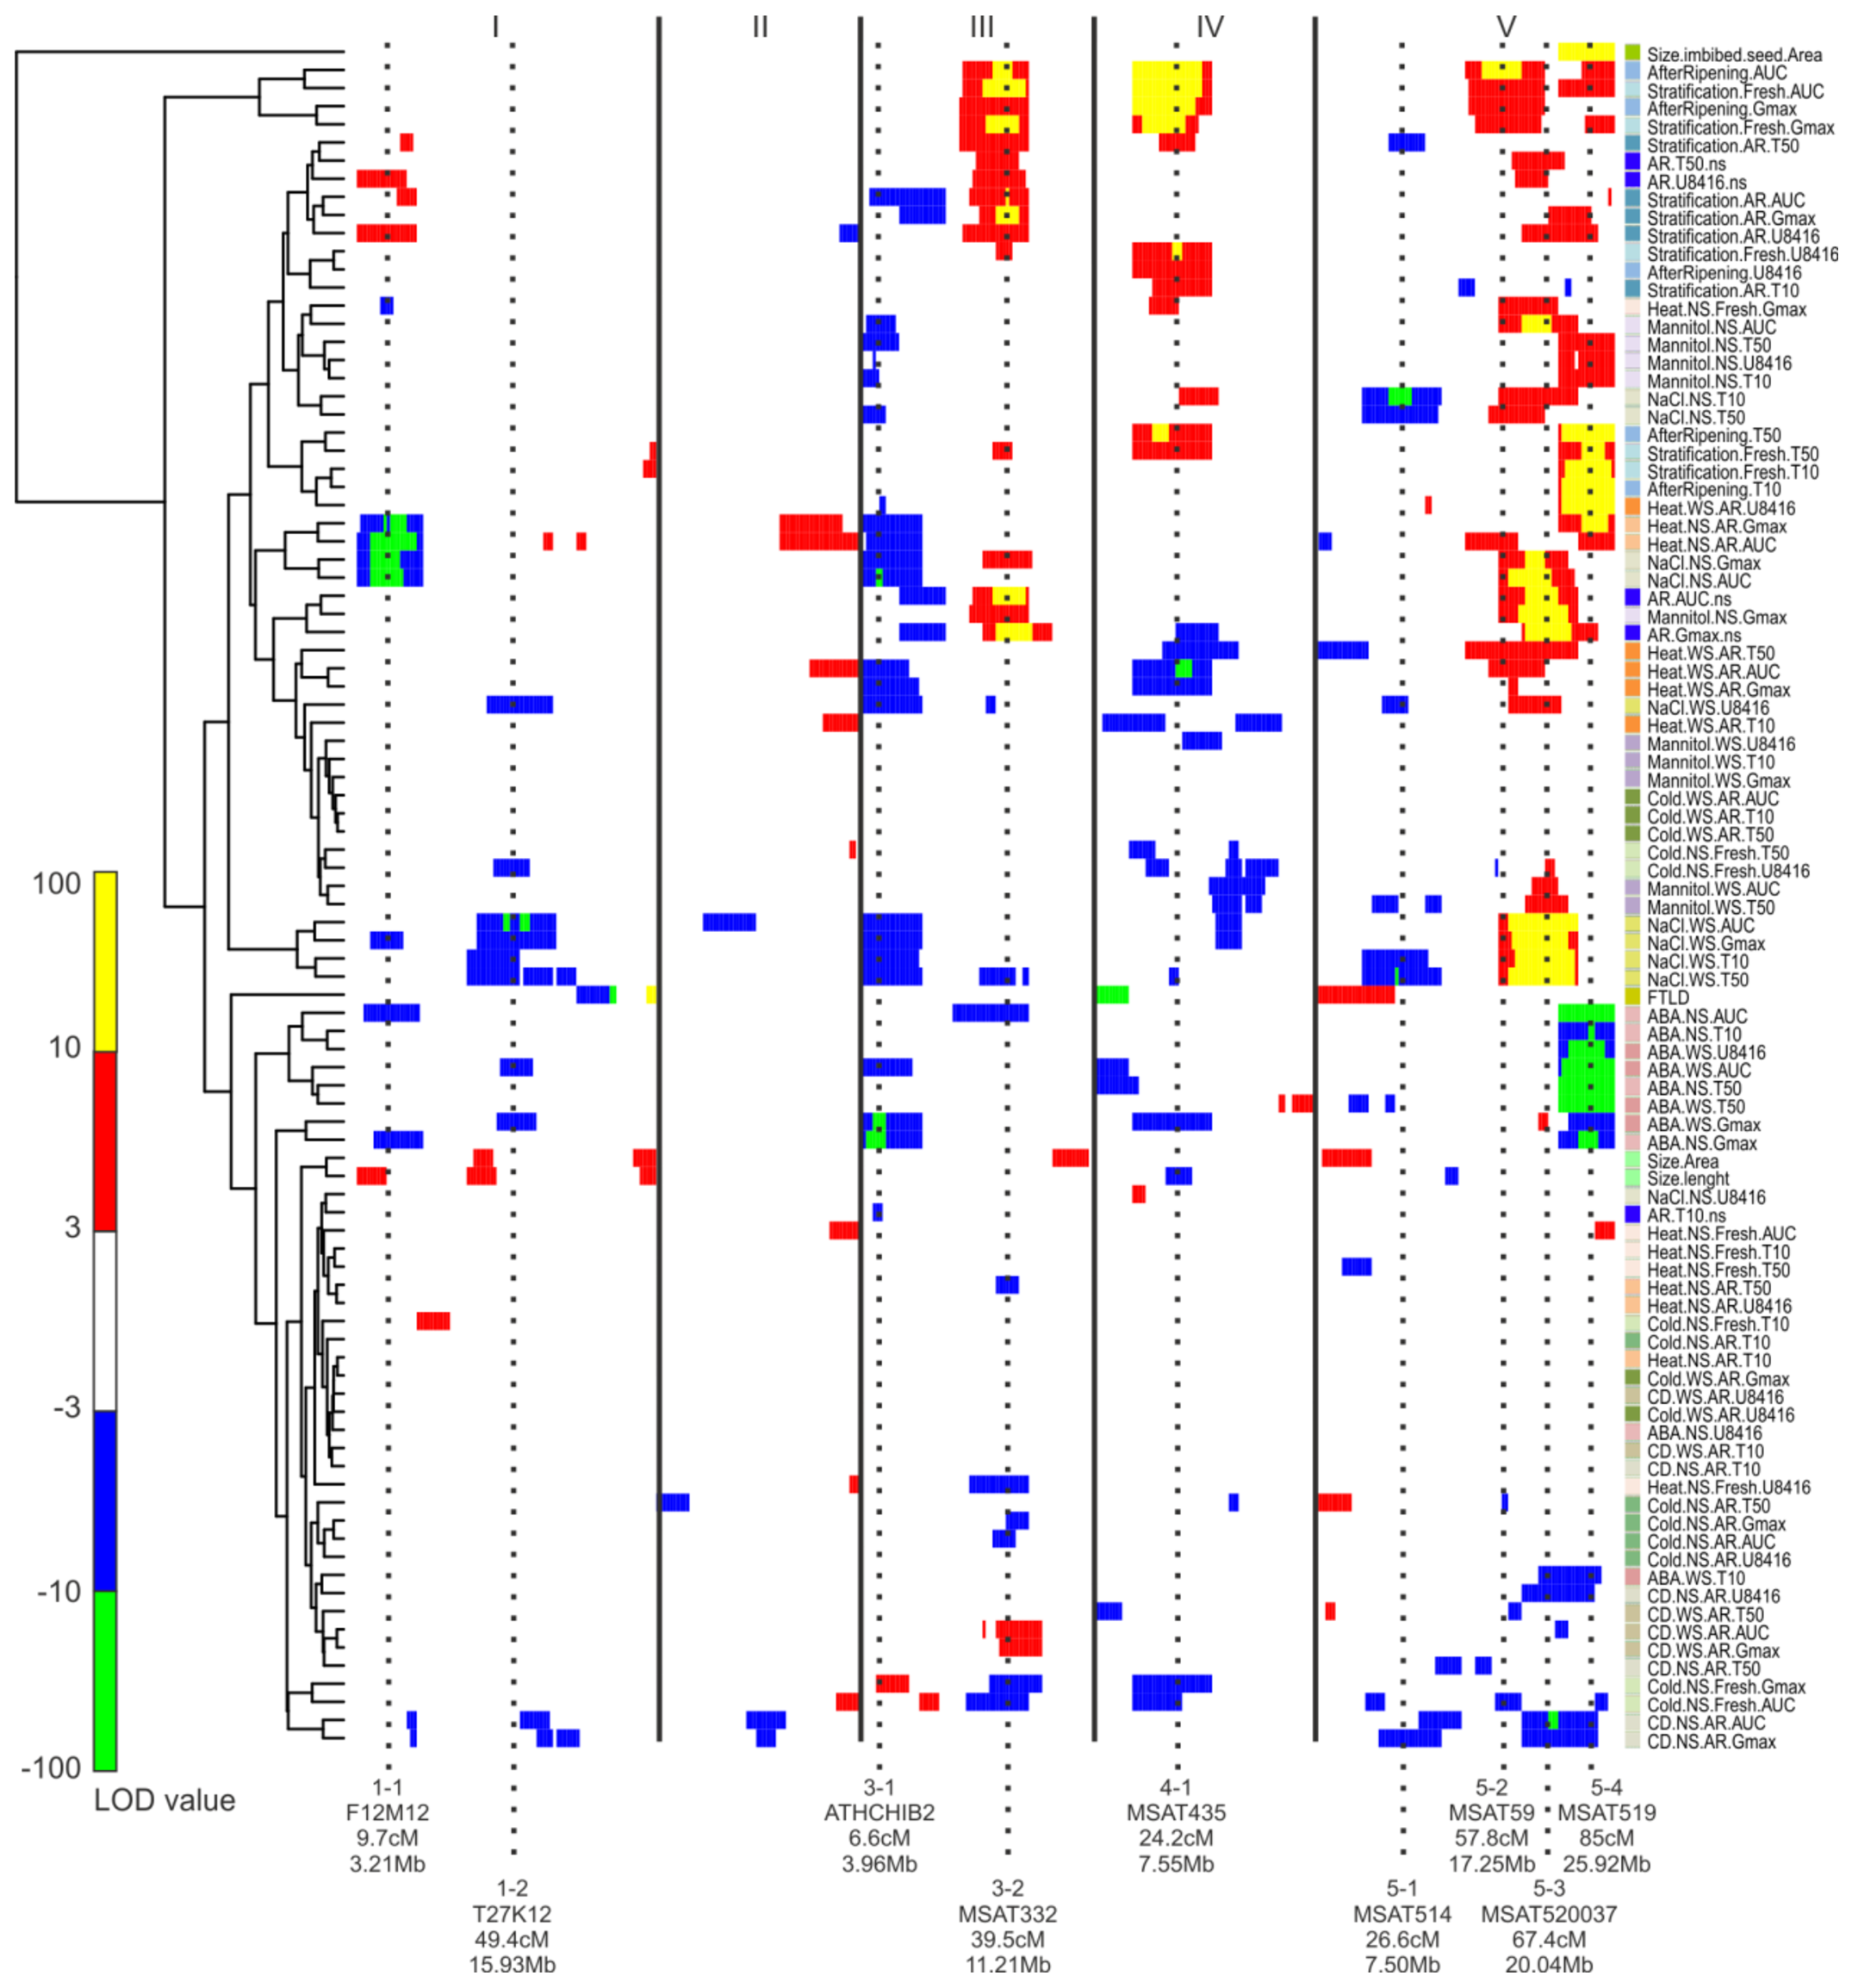
\includegraphics[keepaspectratio,scale=0.30]{eps/image_3_1_4.eps}
  \caption[QTL locations.]{A clustered heat map showing the LOD profiles of the measured traits is automatically 
          produced. Columns indicate chromosome position along the 5 chromosomes; rows indicate individual trait 
          LOD profiles. A false color scale is used to indicate the QTL significance. Positive values (yellow and red) 
          represent a larger effect of the treatment in Shahdara, negative values (blue and green) in Bayreuth..}
\end{figure}

Backward elimination is performed to remove cofactors that do not significantly contribute to the fit 
of the initial model. This is achieved by comparing Akaike's information criterions (AIC) of the 
different models \cite{Jansen:1993}. Using the final selected QTL model, the mapping LOD scores are 
calculated for all genetic markers. Plots showing all significant markers are produced automatically 
(Fig. \ref{fig:generatedoutput}D). We have used the procedure described to map all 327 individual measurements but to enhance
readability we only show average values for each trait (94 traits)

\subsubsection{QTLxQTL Interactions}
Epistatic interactions between QTL can help to elucidate meaningful co-localizations and will enable an 
efficient design of follow up experiments. Besides the visualization of the epistatic interactions per 
trait (Fig. \ref{fig:generatedoutput}F) our script creates an output that can help to visualize all detected epistatic 
interactions in a single plot. This output file in sif format summarizes all detected epistatic 
interactions (Fig. \ref{fig:epistaticinteractions}). Among others, clear hotspots of 
epistatic interactions between QTL loci on chromosome 3, 4 and 5 (resp. ATHCHIB2 + MSAT332, MSAT435 and 
MSAT520037 + MSAT519) were observed for germination on salt (yellow lines) and dormancy (blue lines). 
Next to the importance of detecting possible interacting loci this QTLxQTL analysis provides additional 
arguments for co-locating QTL to be of similar genetic origin. Overall, the creation of this type of 
summarizing figures is greatly facilitating the interpretation of large datasets.

\begin{figure}[h!]
  \centering
  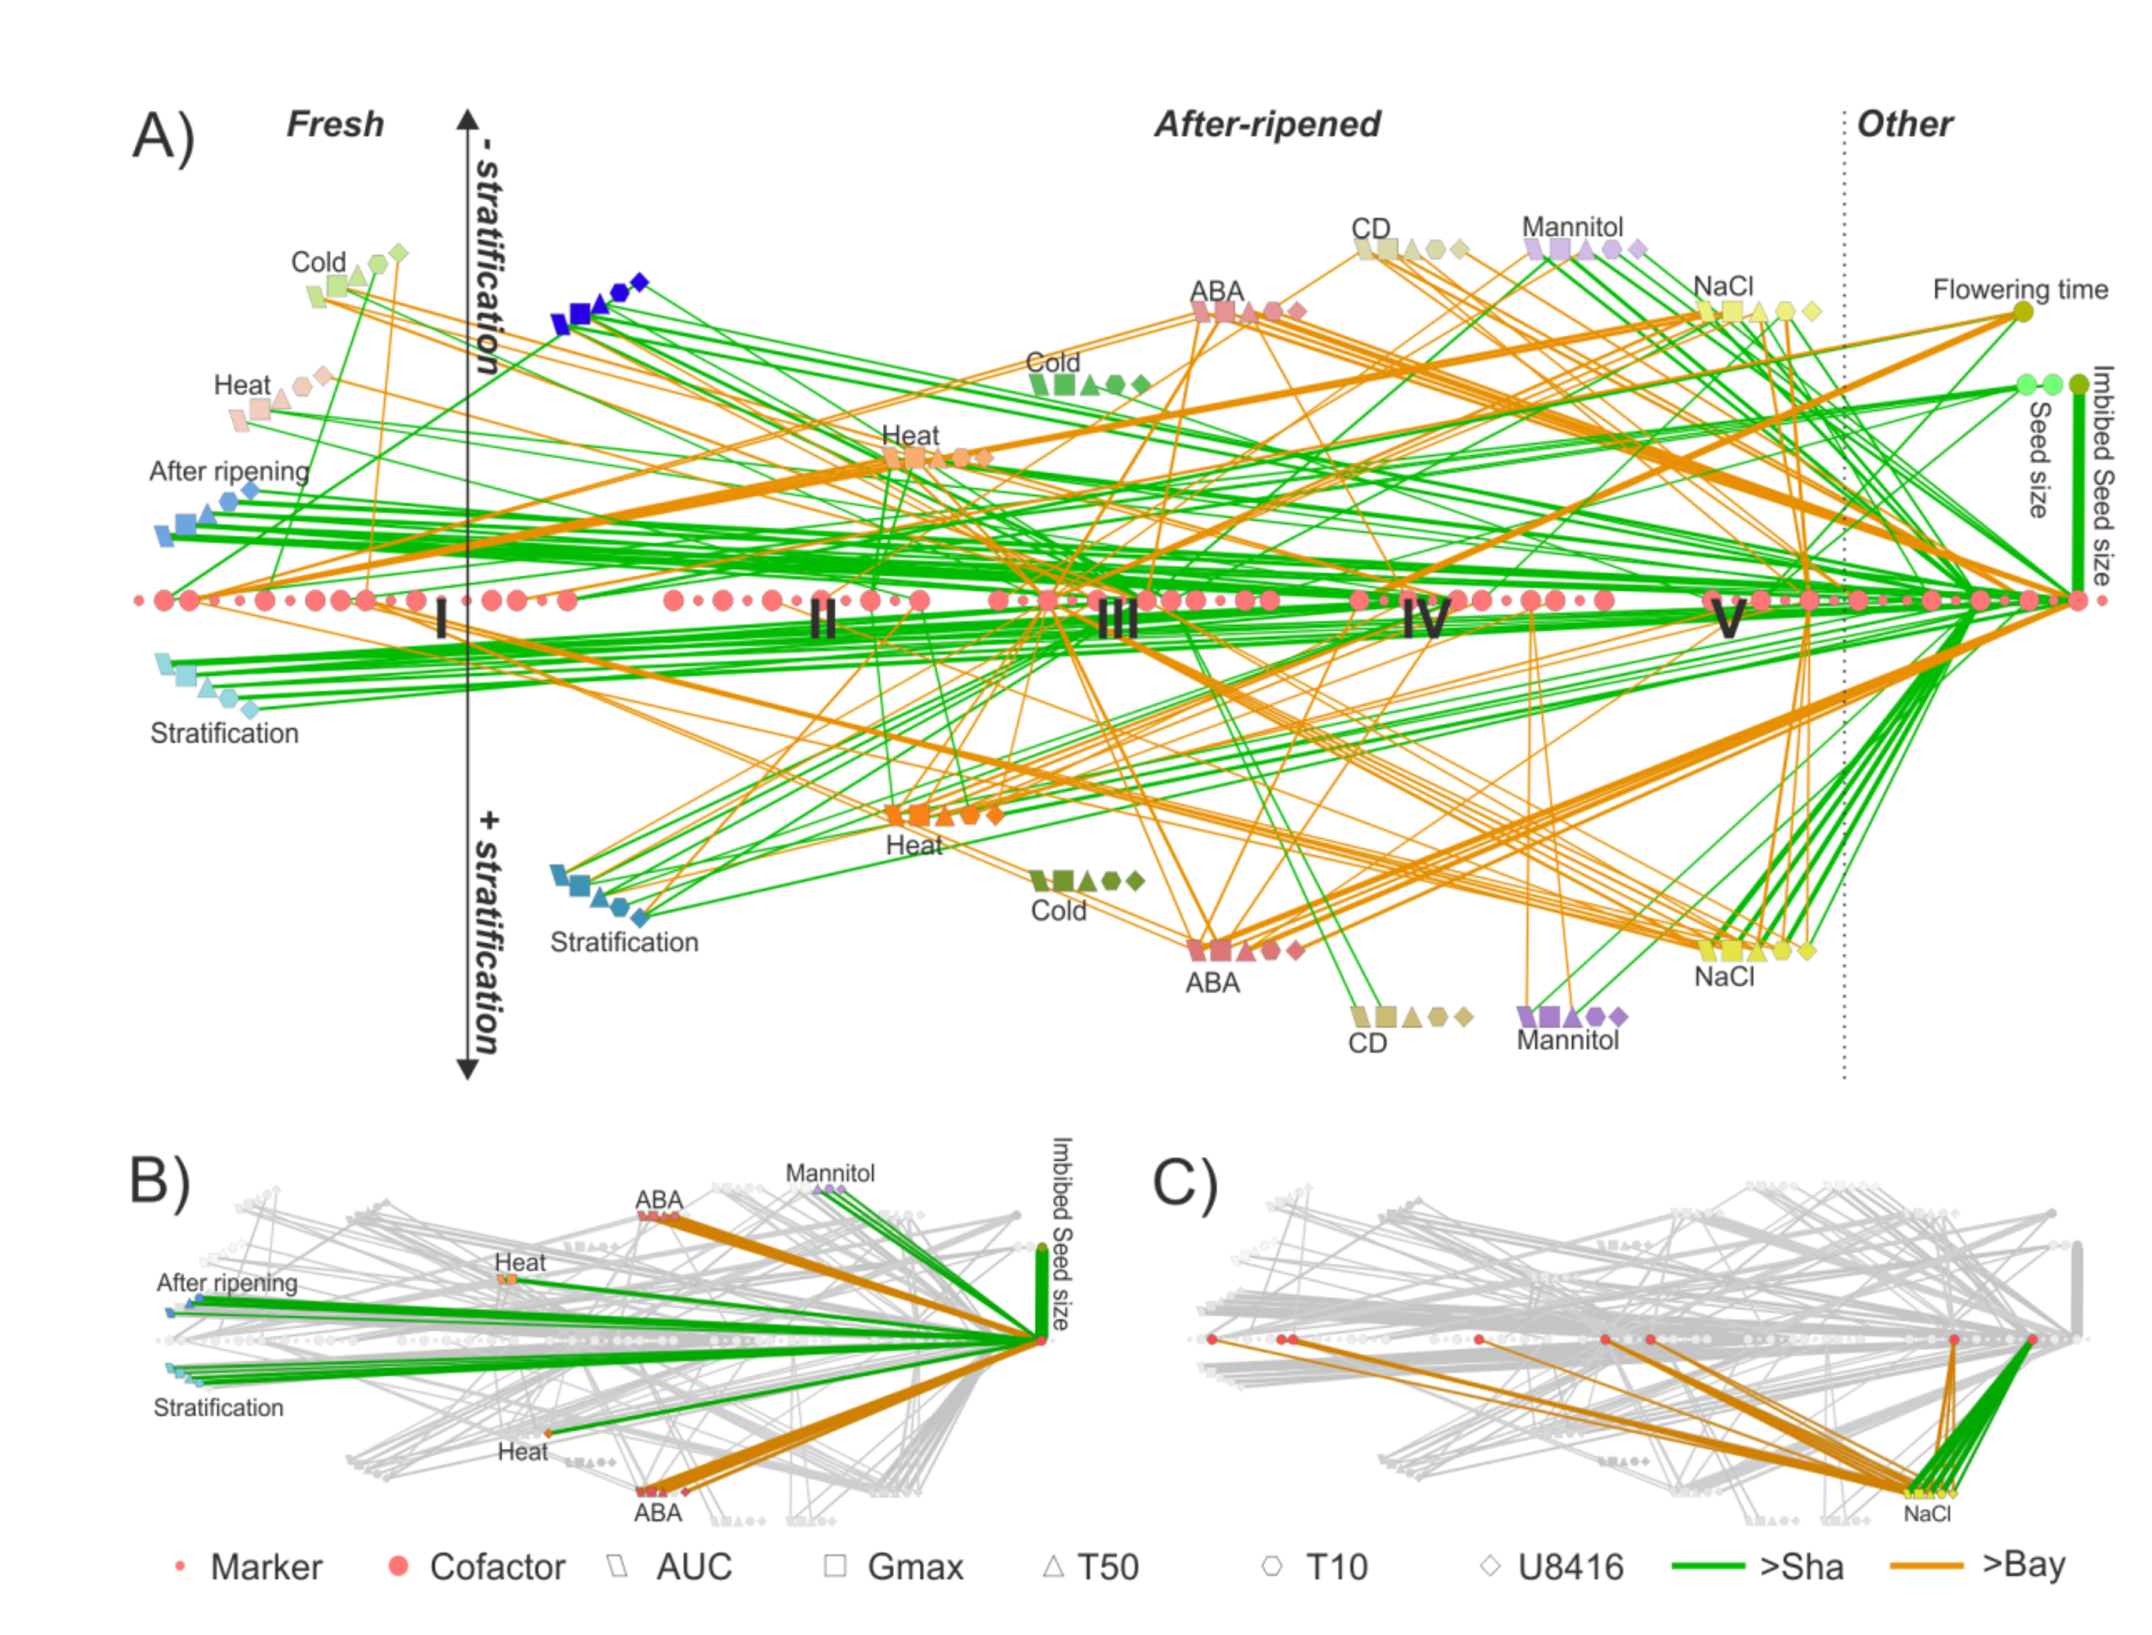
\includegraphics[keepaspectratio,scale=0.30]{eps/image_3_1_5.eps}
  \caption[Cytoscape marker trait network.]{Cytoscape Marker-Trait network. A) Significant QTL positions are 
          indicated by a connection between traits and markers, edge colors indicate the direction of the QTL 
          effect, line width indicates the LOD score; B) Sub- network showing all traits with a significant 
          QTL at marker MSAT519; C) Sub- network showing all markers with significant QTL for germination on 
          NaCl with stratification.}
\end{figure}

\begin{figure}[h!]
  \centering
  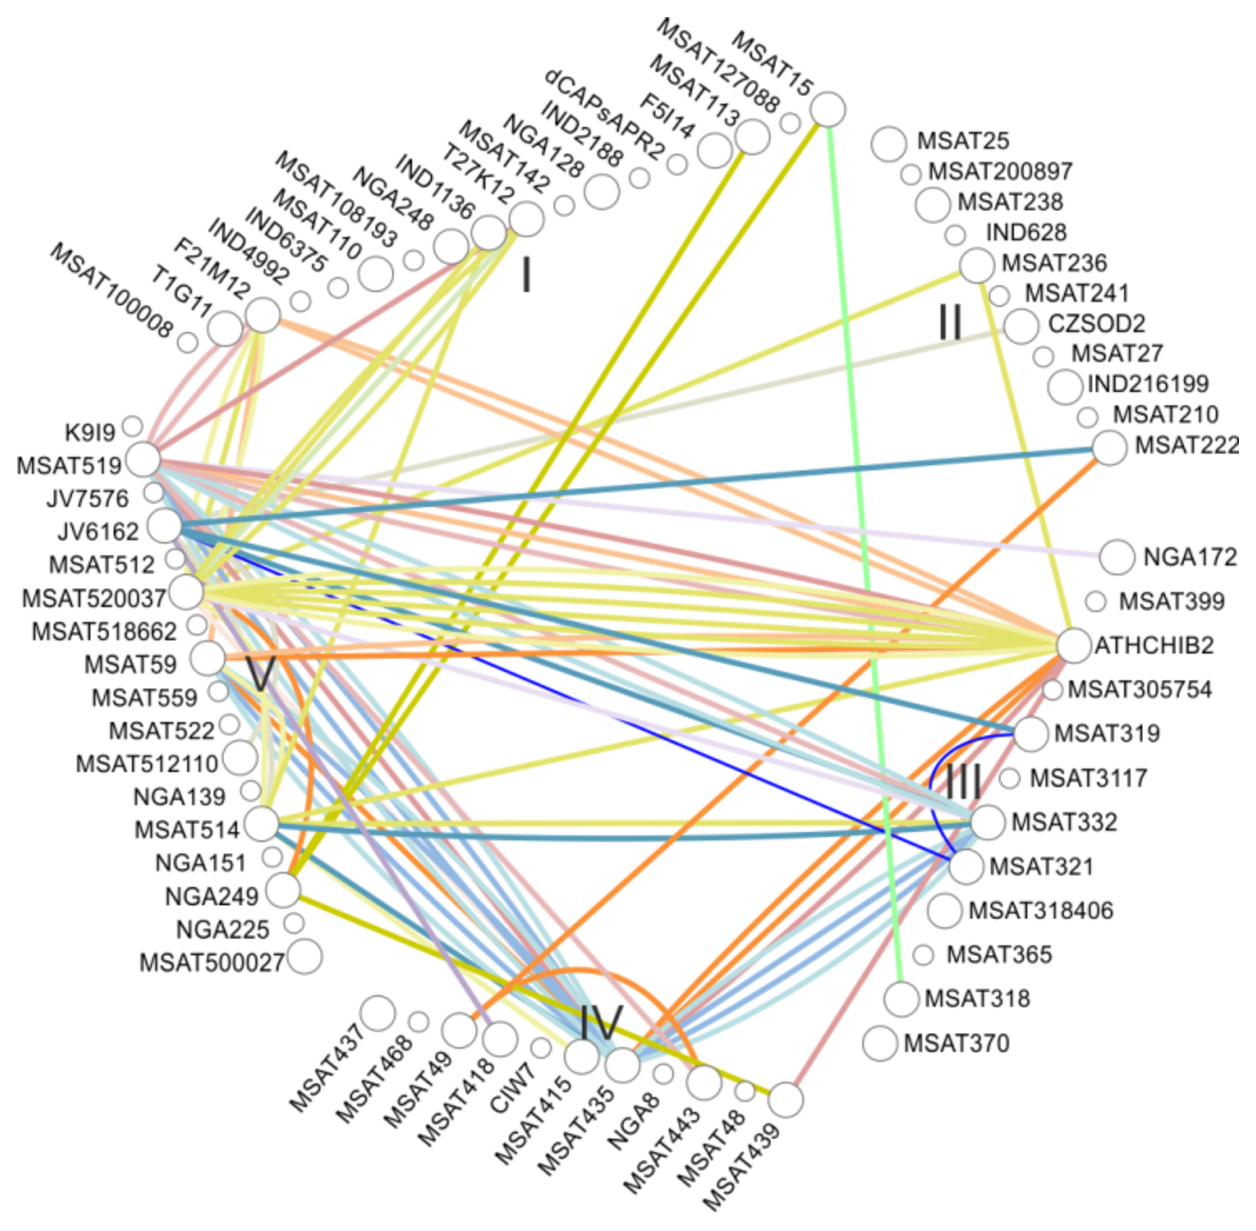
\includegraphics[keepaspectratio,scale=0.30]{eps/image_3_1_6.eps}
  \caption[Epistatic interaction network.]{Epistatic interaction network created with Cytoscape from the 
          interaction.sif output file. Nodes indicate markers (small circles) and selected cofactors (large 
          circles). Edges represent the detected significant epistatic interactions (edge colors represent 
          traits, see table \ref{table:codes} for colors).}
          \label{fig:epistaticinteractions}
\end{figure}

\subsubsection{QTLxEnvironment interaction}
To obtain a parameter for the response, we had to correct all values with their proper control condition 
values. This sometimes led to complex interpretation, which can be circumvented by using the non-corrected 
germination parameters and model them over the various environmental conditions that were tested. Because 
several environments are taken into account simultaneously the statistical power to detect loci that are 
affected by several environments increases and interpretation becomes more intuitive as the need for 
correcting the stress response by the control response is eliminated. By using this approach the 
sensitivity of a specific QTL for environmental conditions can be determined for each separate germination 
parameter. Details about the procedure are described in Material and Methods. Results are summarized in 
figure \ref{fig:gegenomewide}. The final model P-value profiles (top panel, Fig. \ref{fig:gegenomewide}) clearly show the great consistency 
between the 5 germination parameters that we measured. However, a closer look also reveals loci that 
are affecting different germination curve parameters. For example, the QTL on top chromosome 5 is not 
detected by measuring maximum germination but iswell defined when using $t_{50}$ or $t_{10}$ as parameter. As 
expected, the parameter AUC (Area Under the Curve) is outperforming the others as it represents a 
combined value for maximum germination percentage, rate and uniformity. For comparison of the 
environment-specific QTL effects for the 5 different germination parameters (5 lower panels, Fig. \ref{fig:gegenomewide}) 
the effects could be compared with germination under control conditions. For example, after ripened 
seeds without stratification (AR.NS) can guide as reference for the stress treatments (AR.NS.ABA, AR.NS.CD, 
AR.NS.Cold, AR.NS.Heat, AR.NS.Mannitol, AR.NS.NaCl). The same analogy holds true for after ripened seeds
without stratification (AR.NS) and freshly harvested seeds without stratification (Fresh.NS). In this way 
stress specific QTLs on chromosome II and top chromosome III can easily be identified. Interestingly, some 
QTLs, including germination at low temperature (top chromosome I) and germination in the presence of 
exogenous ABA (bottom chromosome V) displayed opposite effects on germination when compared to the 
other treatments.

\begin{figure}[h!]
  \centering
  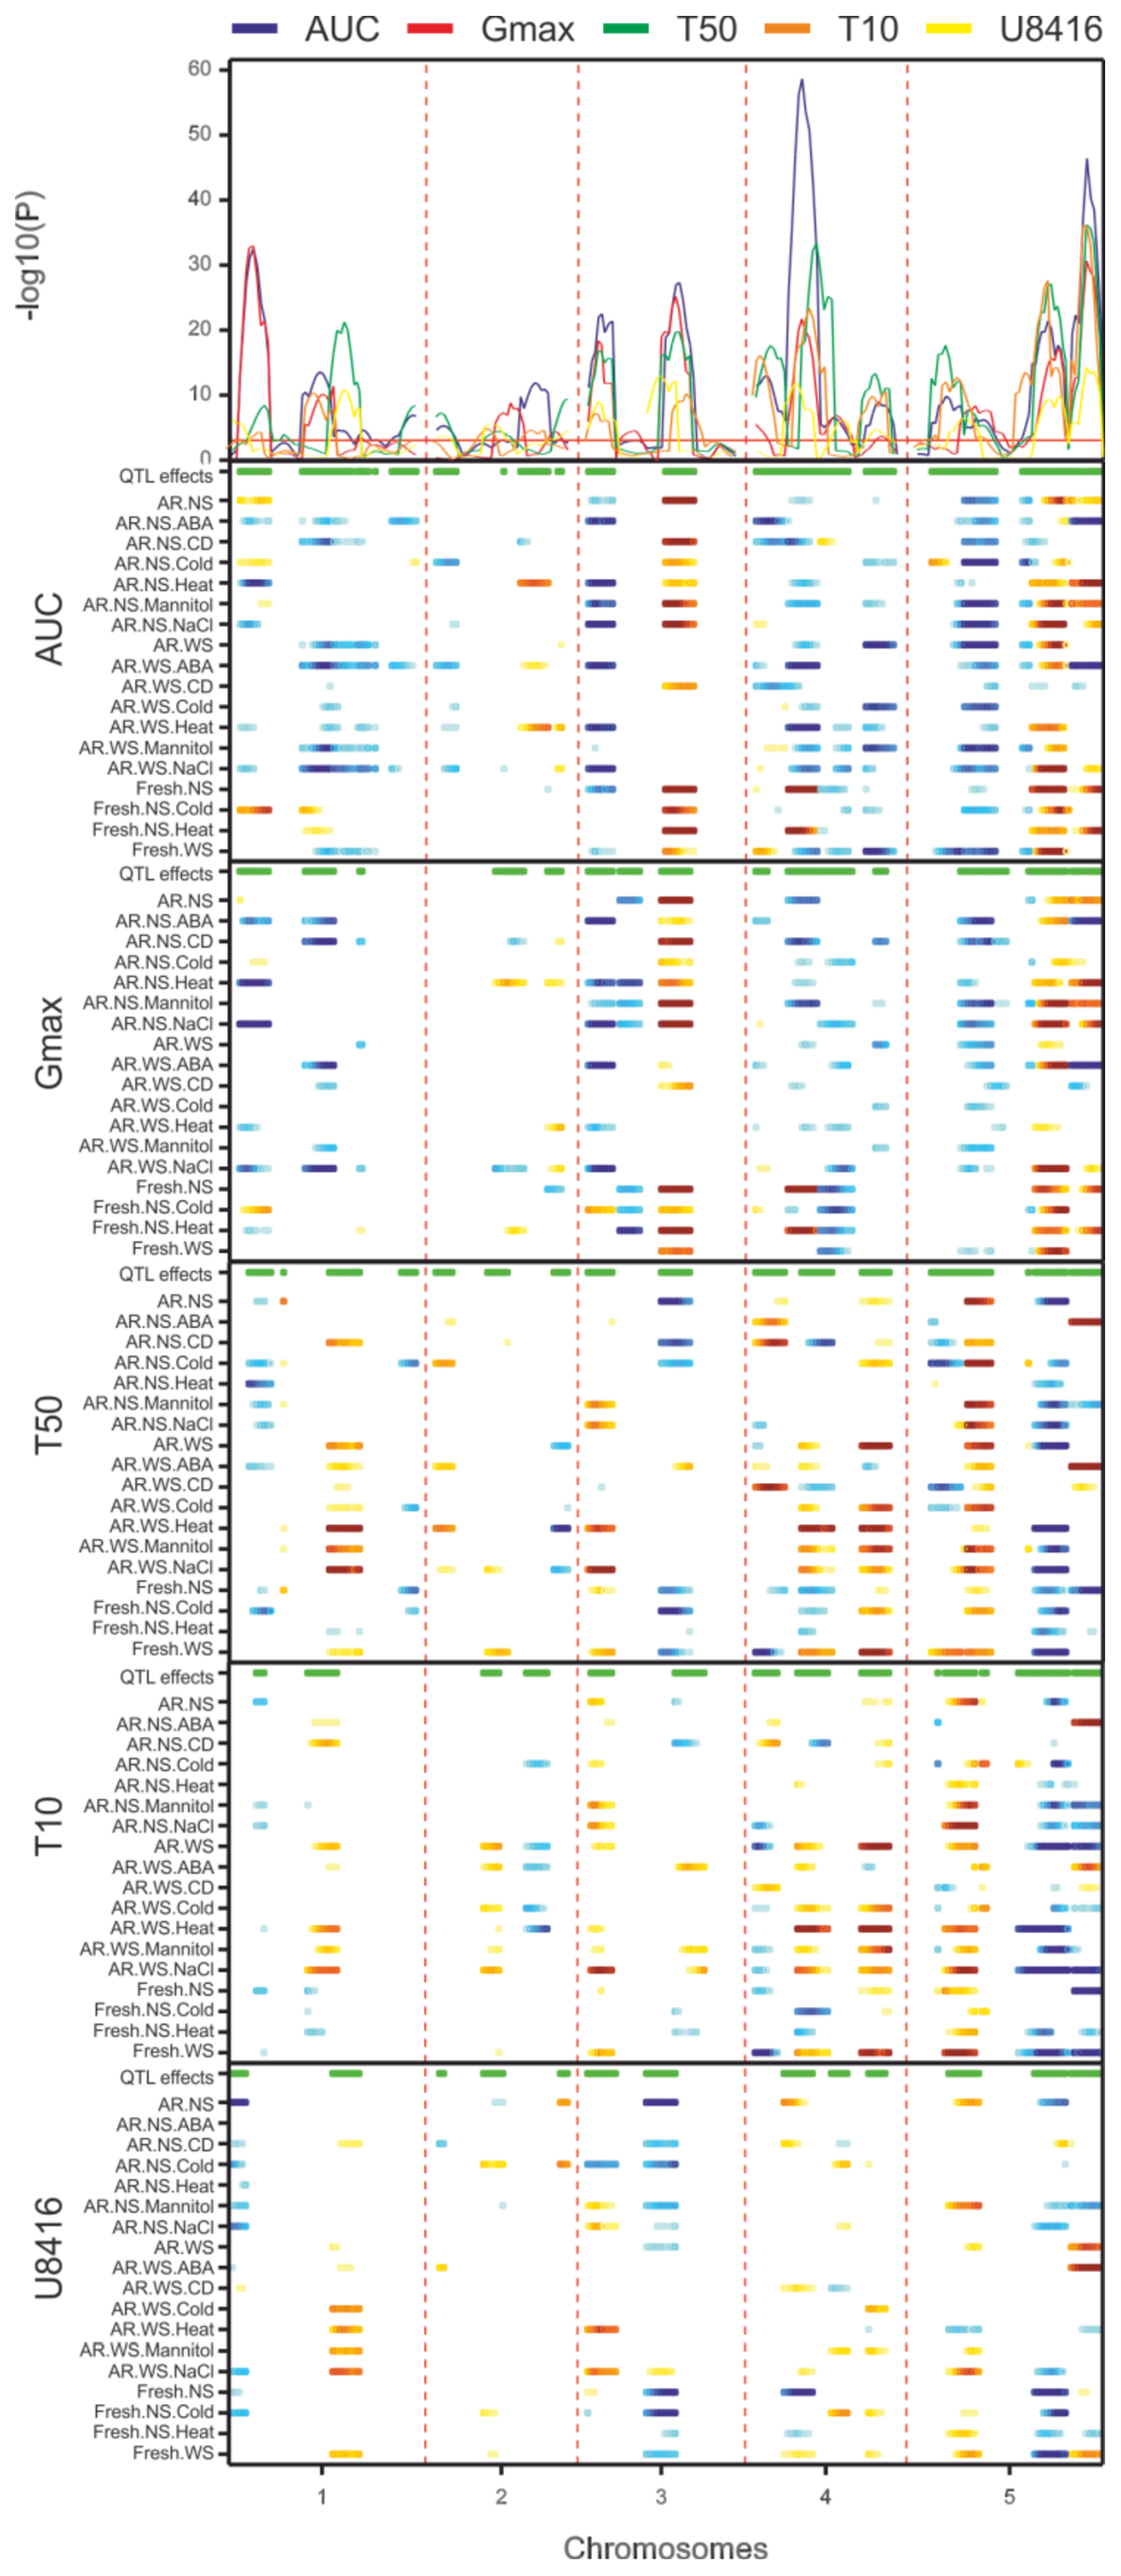
\includegraphics[keepaspectratio,scale=0.30]{eps/image_3_1_7.eps}
  \caption[G:E genome wide QTL scan.]{Genome scan for QTLxEnvironment effects for seed germination. The P-values for 
          the main effects of the different germination parameters are shown in the top panel. The red horizontal line 
          is the genome wide significance threshold. The 5 bottom panels show the environment specific QTL effects. 
          The green line indicates significant environment specific effects. For both Gmax and AUC a bigger effect of 
          the Sha allele is indicated in yellow-red (Bay-0 in cyan-blue). The color scale is opposite for the t50, 
          t10 and U8416 parameters due to the inversed nature of these parameters.}
          \label{fig:gegenomewide}
\end{figure}

\subsubsection{QTL confirmation}
Taking advantage of the residual heterozygosity present in the F6 generation of the Bay-0 x Sha population, 
combined with the large population size, we were able to confirm several QTL following the heterogeneous 
inbred family (HIF) approach. In short, RIL lines which are heterozygous at the locus of interest were 
selected in the next generation for lines homozygous for both parental alleles. These 'families' are 
near isogenic lines (NIL) which can be used to confirm the observed allelic effects (Fig. \ref{fig:confirmation}A). We 
applied this strategy for 7 of the major QTL that we detected in  this study and tested the 5 germination 
parameters for 11 different conditions. For a single parameter (Gmax) and a single HIF (line HIF103) the 
analytical procedure is summarized in figure \ref{fig:confirmation}B. We 
detected a vast QTL for imbibed seed size at the bottom of chromosome 5, which could be confirmed by the 
use of HIF103. Upon imbibition seeds swell due to rapid water uptake and possibly because of the 
expansion of the inner mucilage layer. In Sha, which is a natural mutant for the MUM2 gene 
\cite{Macquet:2007}, this swelling did not occur. Also the HIF lines at the MUM2 position showed a 
clear difference in swelling phenotype which was still significant 24 hours after imbibition (Fig. \ref{fig:swelling}).

\begin{figure}[h!]
  \centering
  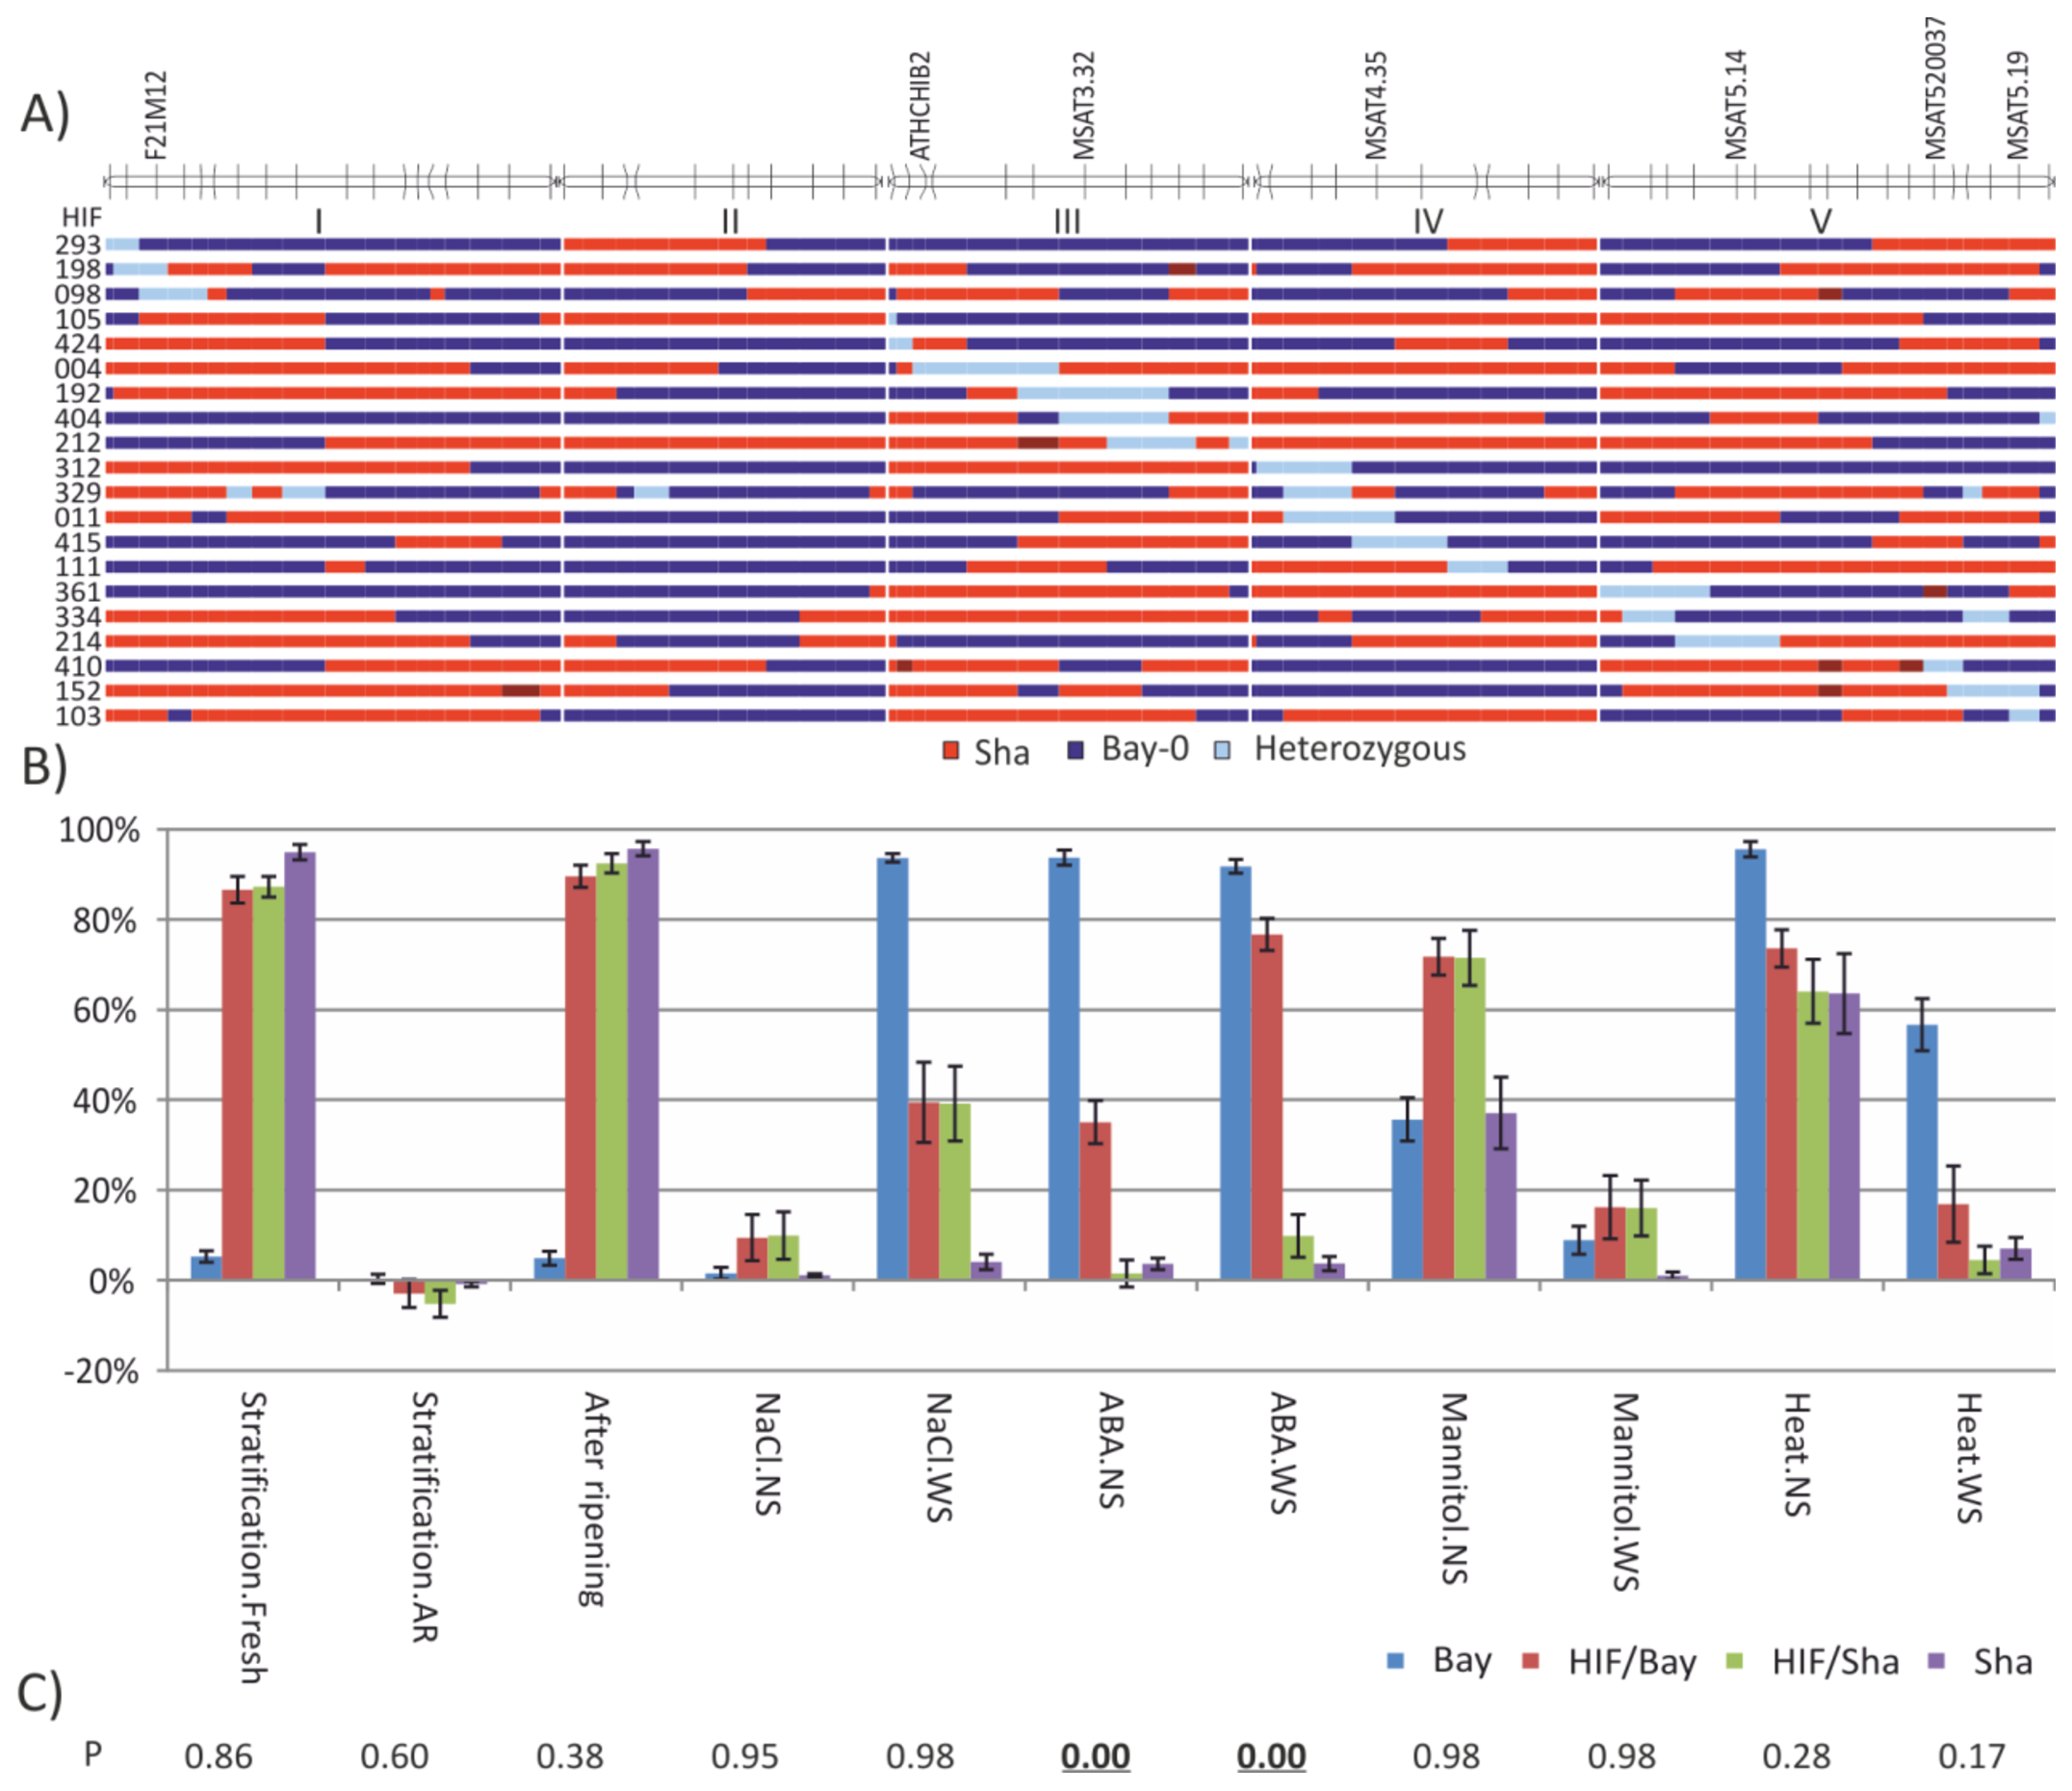
\includegraphics[keepaspectratio,scale=0.30]{eps/image_3_1_8.eps}
  \caption[QTL confirmation.]{Example of the confirmations performed with the HIF approach. A) The blue/red bars 
          indicate the allelic confirmation of the HIF lines used (blue=Bay-0, red=Sha, light blue=segregating). 
          The 5 chromosomes are indicated at the top with the nearest genetic marker for the 7 major loci. B) example 
          analysis for HIF103 (segregating at MSAT5.19, bottom chromosome V). Indicated is the maximum germination 
          (Gmax) for 11 conditions. Error bars represent standard error of at least 6 replicates. Responses are 
          calculated by subtracting the test sample from the control sample as indicated in table \ref{table:codes}. C) T-test 
          significance values for the response values (significant (P<0.05) values are bold).}
          \label{fig:confirmation}
\end{figure}

\begin{figure}[h!]
  \centering
  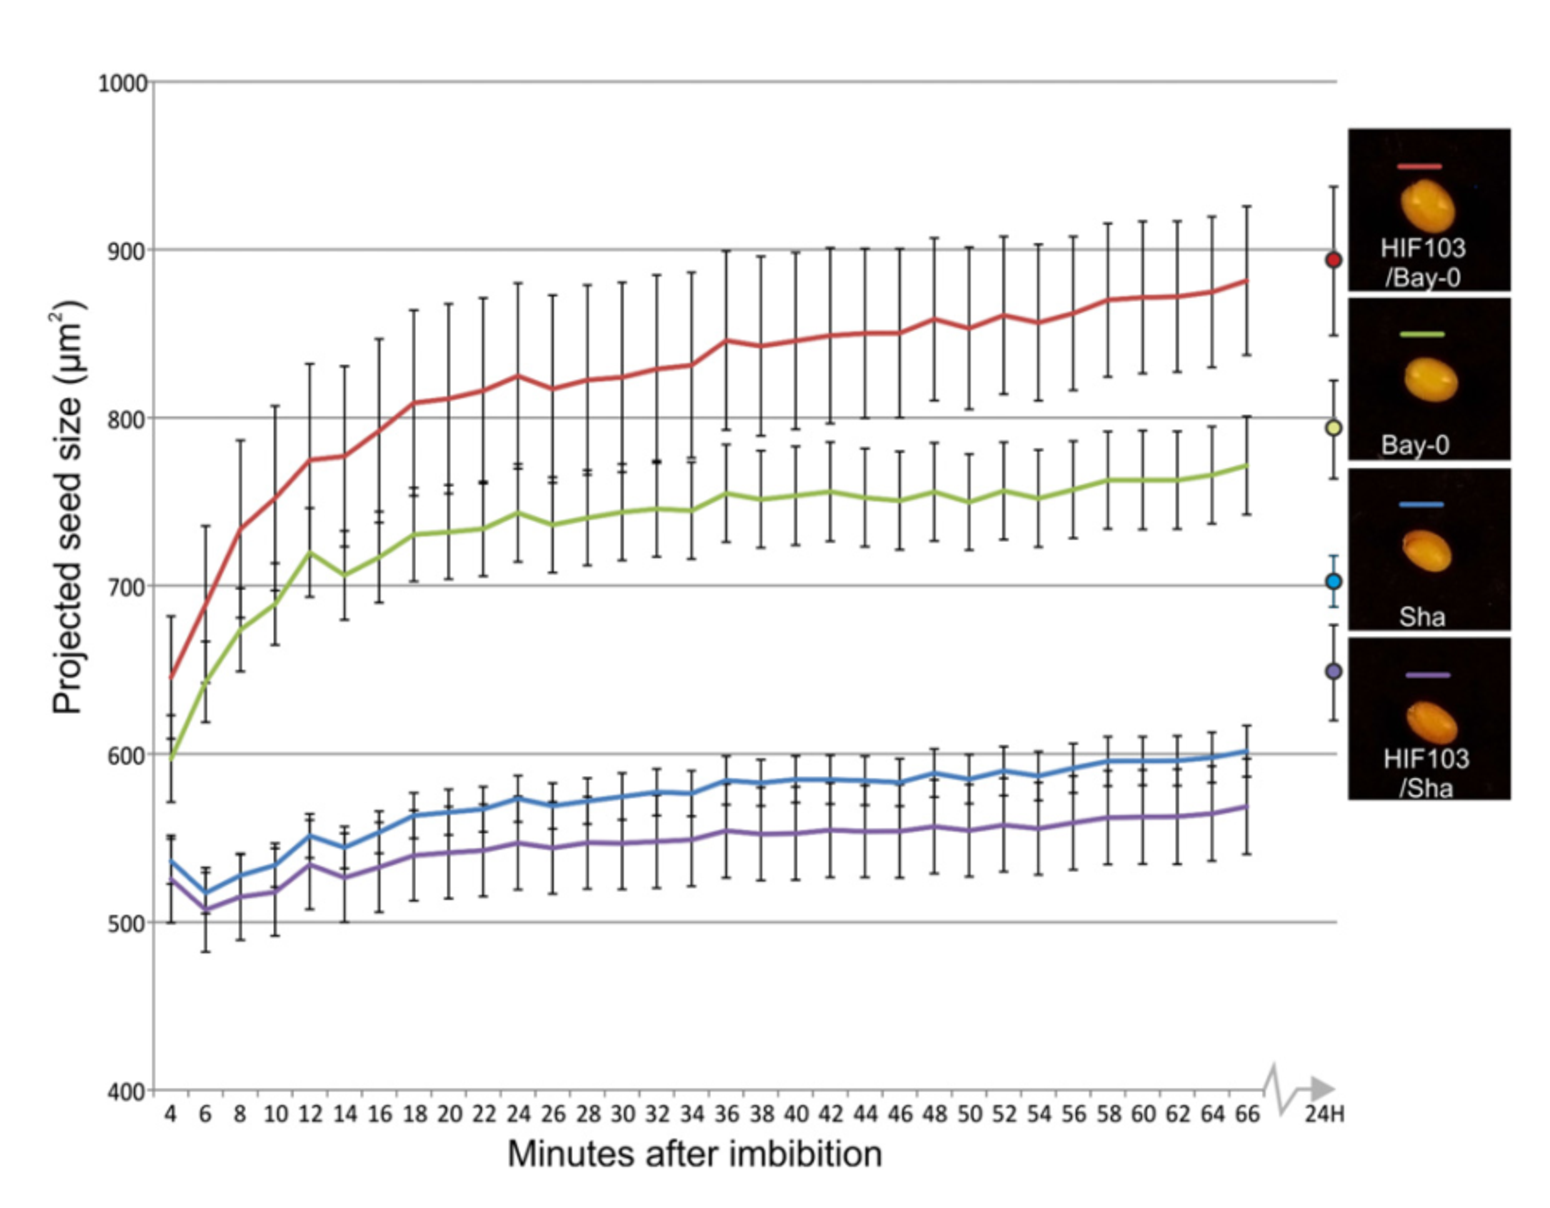
\includegraphics[keepaspectratio,scale=0.30]{eps/image_3_1_9.eps}
  \caption[Seed Swelling.]{Different increases in seed size during the start of imbibition for Bay-0 (green), Sha (blue), 
          HIF103/Bay-0 (red), and HIF103/Sha (purple) seeds. Shown is the average projected seed size area of 10 seeds. 
          Error bars represent SE values. Photographs show 24-h imbibed seeds.}
          \label{fig:swelling}
\end{figure}

\subsection{Conclusions and Discussion}
When analyzing large (RIL) populations, it is hardly feasible to manually count all germination 
experiments several times a day to obtain germination curves. Therefore, previous studies mostly 
restricted to counting end-point germination \cite{Quesada:2002, Alonso-Blanco:2003, Clerkx:2004, 
Laserna:2008, Meng:2008, Bentsink:2010, Galpaz:2010, Vallejo:2010}. A germination curve allows QTL 
mapping under conditions where rate and uniformity are delayed, but maximum germination is not 
affected. Therefore, we used the Germinator package \cite{Joosen:2010} that enabled measurement 
of cumulative germination data and extracting 5 germination parameters that describe the resulting 
germination curve. In the present study we describe several germination QTLs that were not detected 
before in the Bay-0 x Sha population. We observed interesting co-localizations for several germination 
traits and identified the loci that show large effect epistatic interactions. Among these were new 
loci and loci similar to the ones already found in other RIL populations (see \cite{Joosen:2011} - Table 4 for 
the major identified QTL loci).

\subsubsection{Dormancy}
Primary dormancy has been studied extensively in various RIL populations \cite{Bentsink:2010}. These 
authors quantified primary dormancy with the DSDS50 parameter (days of dry storage to reach 50\% 
germination), which is a good measure for after-ripening related dormancy breaking. Although we only 
compared the germination characteristics of freshly harvested seeds with those of after ripened 
seeds and fresh seeds with and without stratification, we detected large genetic variation. Both 
dormancy breaking treatments showed strong QTL at positions 3-2, 4-1 and 5-2, co-locating with DOG6, 
DOG18 and DOG1, respectively (See \cite{Joosen:2011} - Table 4). DOG18 was not detected in a LerxSha population and showed a 
stronger dormancy in Ler as compared with An-1, Fei-0 and Kas-2 \cite{Bentsink:2010}. We detected stronger 
dormancy in Sha as compared to Bay-0 at the DOG18 locus. This suggests that both Ler and Sha contain 
an allele of similar strength which is stronger when compared to An-1, Fei-0,  Kas-2 and Bay-0. Remarkably, 
for both the DOG6 and DOG18 location the sensitivity to ABA was higher in Bay-0, whereas dormancy was 
deeper in Sha, which resulted in a directional change of the QTL effect. The more dormant Sha parent 
contains higher initial ABA levels and apparently, after-ripening and 
stratification reduce the ABA sensitivity to a greater extent as compared to the Bay-0 parent. This 
effect was not observed for the DOG1 locus. Further, we identified a strong effect of the dormancy-
breaking treatments on the initiation (t10) and rate (t50) of germination at the bottom of chromosome 5 
(marker MSAT519, 85 cM). The same was observed for germination on mannitol and germination at higher 
temperature. A QTL with opposite effect at this position was found for germination on ABA. Interestingly, 
these co-located with a QTL found for imbibed seed size. 

\subsubsection{Water uptake}
Initiation and rate of germination are highly influenced by the overall water potential of the seed. The 
mucilage layer surrounding the seed appears to play an important role in the process of water uptake 
\cite{Penfield:2001}. Sha is a natural mucilage mutant due to a mutation in the MUM2 gene, which changes 
the hydrophilic potential of rhamnogalacturonan I \cite{Macquet:2007}. Although mucilage has been reported 
to be dispensable for germination and development under lab conditions \cite{Arsovski:2010}, a link with 
germination under reduced water potential conditions was shown by \cite{Penfield:2001}. They showed 
reduced maximum germination of a mucilage-impaired mutant only on osmotic PEG solutions. In our study, 
other traits that co-located on the MUM2 locus were delayed initiation and rate of germination on osmotic
mannitol solution but also on water, which clearly shows the advantage of determining a detailed 
germination curve. We also observed a very strong QTL for swelling of the seed in the first hours of 
imbibition (imbibed seed size) at the MUM2 location. Interestingly, exogenous ABA can be used to 
stimulate mucilage production and ABA-1 mutants are affected in mucilage production \cite{Karssen:1989}. 
This indicates a regulatory role of ABA in mucilage production and fits with our observation of the 
co-localization of a QTL for initiation and rate of germination with a QTL with opposite effect for ABA 
sensitivity. Therefore, we hypothesize that Sha has a slower initiation and rate of germination,
combined with reduced ABA sensitivity due to its mutation in the MUM2 gene. This observation may open 
new research strategies to define the regulatory role of ABA in mucilage production and its multiple 
effects on germination parameters.

\subsubsection{Salt, Heat and ABA}
At the top of chromosome I, underlying marker F12M12, we detected a strong QTL for maximum germination in 
the presence of 100 mM NaCl or 0.5μm ABA. A similar locus has been identified and fine-mapped in a 
LerxSha population \cite{Ren:2010}. They identified a premature stop codon in the Response to ABA and 
Salt 1 gene (RAS1; At1g09950) in Sha that led to a truncated protein and showed its role as a negative 
regulator of salt tolerance during seed germination and early seedling growth by enhancing ABA 
sensitivity. Here we show that a similar locus is also inferring tolerance to germination at 30\degree C. 
This suggests an additional role for the RAS1 gene. Increased heat tolerance due to modulation of 
ABA sensitivity has been shown before for other loci, \cite{Argyris:2008,Lee:2010}. 
Interestingly, our present study showed a strong effect of stratification which resulted in a strong 
reduction of significant linkage for NaCl, heat and ABA sensitivity at the F12M12 locus. A specific 
QTL for germination on NaCl preceded by a cold stratification period was found at the middle of 
chromosome I (marker T27K12). Also at this locus we found colocation with sensitivity for germination 
on ABA after stratification. Further fine-mapping at this locus might help to elucidate the effect 
of stratification on ABA mediated abiotic stress tolerance, as well as the apparent overlap of 
dormancy and stress responses. Especially interesting is QTL 5-1 (See \cite{Joosen:2011} - Table 4, and Fig. \ref{fig:gegenomewide}) which mainly 
influences rate and initiation of germination. We detected this QTL for t50 in after ripened seeds 
with stratification treatment, but also for t10 and t50 for germination on salt, regardless of a 
preceding cold stratification and for maximum germination after an accelerated aging treatment. 
One of the genes underlying this QTL interval is a nicotinamidase gene (NIC2, At5g23230), the mutant 
of which has retarded germination and impaired germination potential \cite{Hunt:2007}. These 
authors suggested that NIC2 is normally metabolizing nicotinamide during moist chilling or 
after-ripening, which relieves inhibition of poly(ADP-ribose) polymerase (PARP enzyme) activity and 
allows DNA repair to occur prior to germination. Both accelerated aging and germination under salt 
stress conditions might require optimal functioning of this DNA repair mechanism. Further research 
is needed to determine whether NIC2 is causal for this QTL.

Detection of epistatic interactions in genetic studies can enhance the understanding of underlying 
molecular mechanisms. Recently, \cite{Galpaz:2010} showed strong epistasis in the genetic network 
controlling germination under salt stress in Arabidopsis. Due to careful dissection of the epistatic 
relationships they were able to show that three detected QTL rely on the presence of a Columbia 
allele at a QTL on top of chromosome 1. This observation led to the hypothesis that RAS1 
\cite{Ren:2010} functions as a switch of the genetic network by regulating the expression of the 
other QTL. In another study it was found that epistasis significantly influences both fitness and 
germination in Arabidopsis \cite{Huang:2010} and novel allele combinations were identified that 
resulted in higher fitness. In our study we detected clear hotspots of epistatic interactions 
between QTL loci on chromosome 3, 4 and 5 (ATHCHIB2, MSAT332, MSAT435, MSAT520037 + MSAT519, 
respectively). This observation strengthens the hypothesis that some of the traits with strong 
QTL co-localizations indeed rely on the same underlying genetic networks.

\subsubsection{Concluding remarks}
We analyzed natural variation for many seed germination characteristics and showed their correlation, 
(shared) QTL positions and epistatic interactions, using a high-throughput phenotyping approach and 
subsequent high-throughput QTL mapping. Using the HIF approach, confirmation of some major QTL 
hotspots was demonstrated, which allows a fast but solid confirmation of a QTL position. Together 
with results from several other studies focusing on genetic variation in seed traits, this study 
has generated an extensive QTL database for Arabidopis and proposed a method of analysis to 
visualize the genetic landscape of seed performance. This database is a solid resource for further 
study. For most of the found loci in this and other studies further characterization, and in most 
cases fine mapping, must be undertaken to elucidate the causal molecular mechanisms. Further, we 
have designed a free available analysis protocol to perform detailed high-throughput QTL analysis 
based on the R/qtl MQM routine. In this era of large-scale phenotyping we regard a detailed analysis 
of QTL, QTLxQTL and QTLxEnvironment interaction as indispensable steps to allow visualization 
and interpretation of multiple traits.

